The data and MC samples used in this analysis are the same 
as in the SM Higgs search analysis~\cite{HWWHCP2012}, with 
the exception of the signal samples. 
The $gg\to X\to WW$ signal samples are generated by JHUGen 
MC generator~\cite{jhugen} with the matrix elements 
calculated at the LO. The generated LHE files are then 
interfaced to PYTHIA for showering, hadronization, and underlying event. 
To validate the JHUGen samples we compare the main kinematic distributions to 
MCFM at the generator level and to Powheg-Pythia at the reconstruction level. 

%%%%%%%%%%%%%%%%%%%%%%%%%%%%%%%%%%%%%%%%%%%%%
\begin{table}[!ht]
\begin{center}
{\footnotesize
\begin{tabular}{|c|c|}
\hline
\multicolumn{2}{|c|}{With Pileup: Processed dataset name is always} \\
\multicolumn{2}{|c|}{/Summer12\_DR53X-PU\_S10\_START53\_V7A-v*/AODSIM} \\ 
\hline
 Dataset Description              		&   Primary Dataset Name  \\ 
\hline
$gg\to H\to WW\to (l\nu)(l\nu)$, $l=e,\mu$      & SMHiggsToWWTo2L2Nu\_M-125\_8TeV-jhu-pythia6 \\ 
$gg\to H\to WW\to (l\nu)(\tau\nu)$, $l=e,\mu$   & SMHiggsToWWToLTau2Nu\_M-125\_8TeV-jhu-pythia6 \\
$gg\to H\to WW\to (\tau\nu)(\tau\nu)$           & SMHiggsToWWToTauTau2Nu\_M-125\_8TeV-jhu-pythia6 \\
$gg\to \text{Graviton}\to WW\to (l\nu)(l\nu)$, $l=e,\mu$      & Graviton2PMToWWTo2L2Nu\_M-125\_8TeV-jhu-pythia6 \\ 
$gg\to \text{Graviton}\to WW\to (l\nu)(\tau\nu)$, $l=e,\mu$   & Graviton2PMToWWToLTau2Nu\_M-125\_8TeV-jhu-pythia6 \\
$gg\to \text{Graviton}\to WW\to (\tau\nu)(\tau\nu)$           & Graviton2PMToWWToTauTau2Nu\_M-125\_8TeV-jhu-pythia6 \\
\hline
\hline
\end{tabular}
}
\caption{Summary of additional Monte Carlo datasets used.\label{tab:DatasetsMC}. }
\end{center}
\end{table}
%%%%%%%%%%%%%%%%%%%%%%%%%%%%%%%%%%%%%%%%%%%%%

Figure~\ref{fig:jhuvsmcfm} compares the main kinematic observables at generator 
level between the JHUGen and MCFM for events without any cuts. 
Both samples are generated with Higgs produced at rest. 
And we observe good agreement within a few \% in the bulk of the distributions between the two. 


%%%%%%%%%%%%%%%%%%%%%%%%%%%%%%%%%%%%%%%%%%%%%
\begin{figure}[!hbtp]
\centering
\subfigure[Leading Lepton $p_T$]{
\centering
\label{subfig:leadleppt}
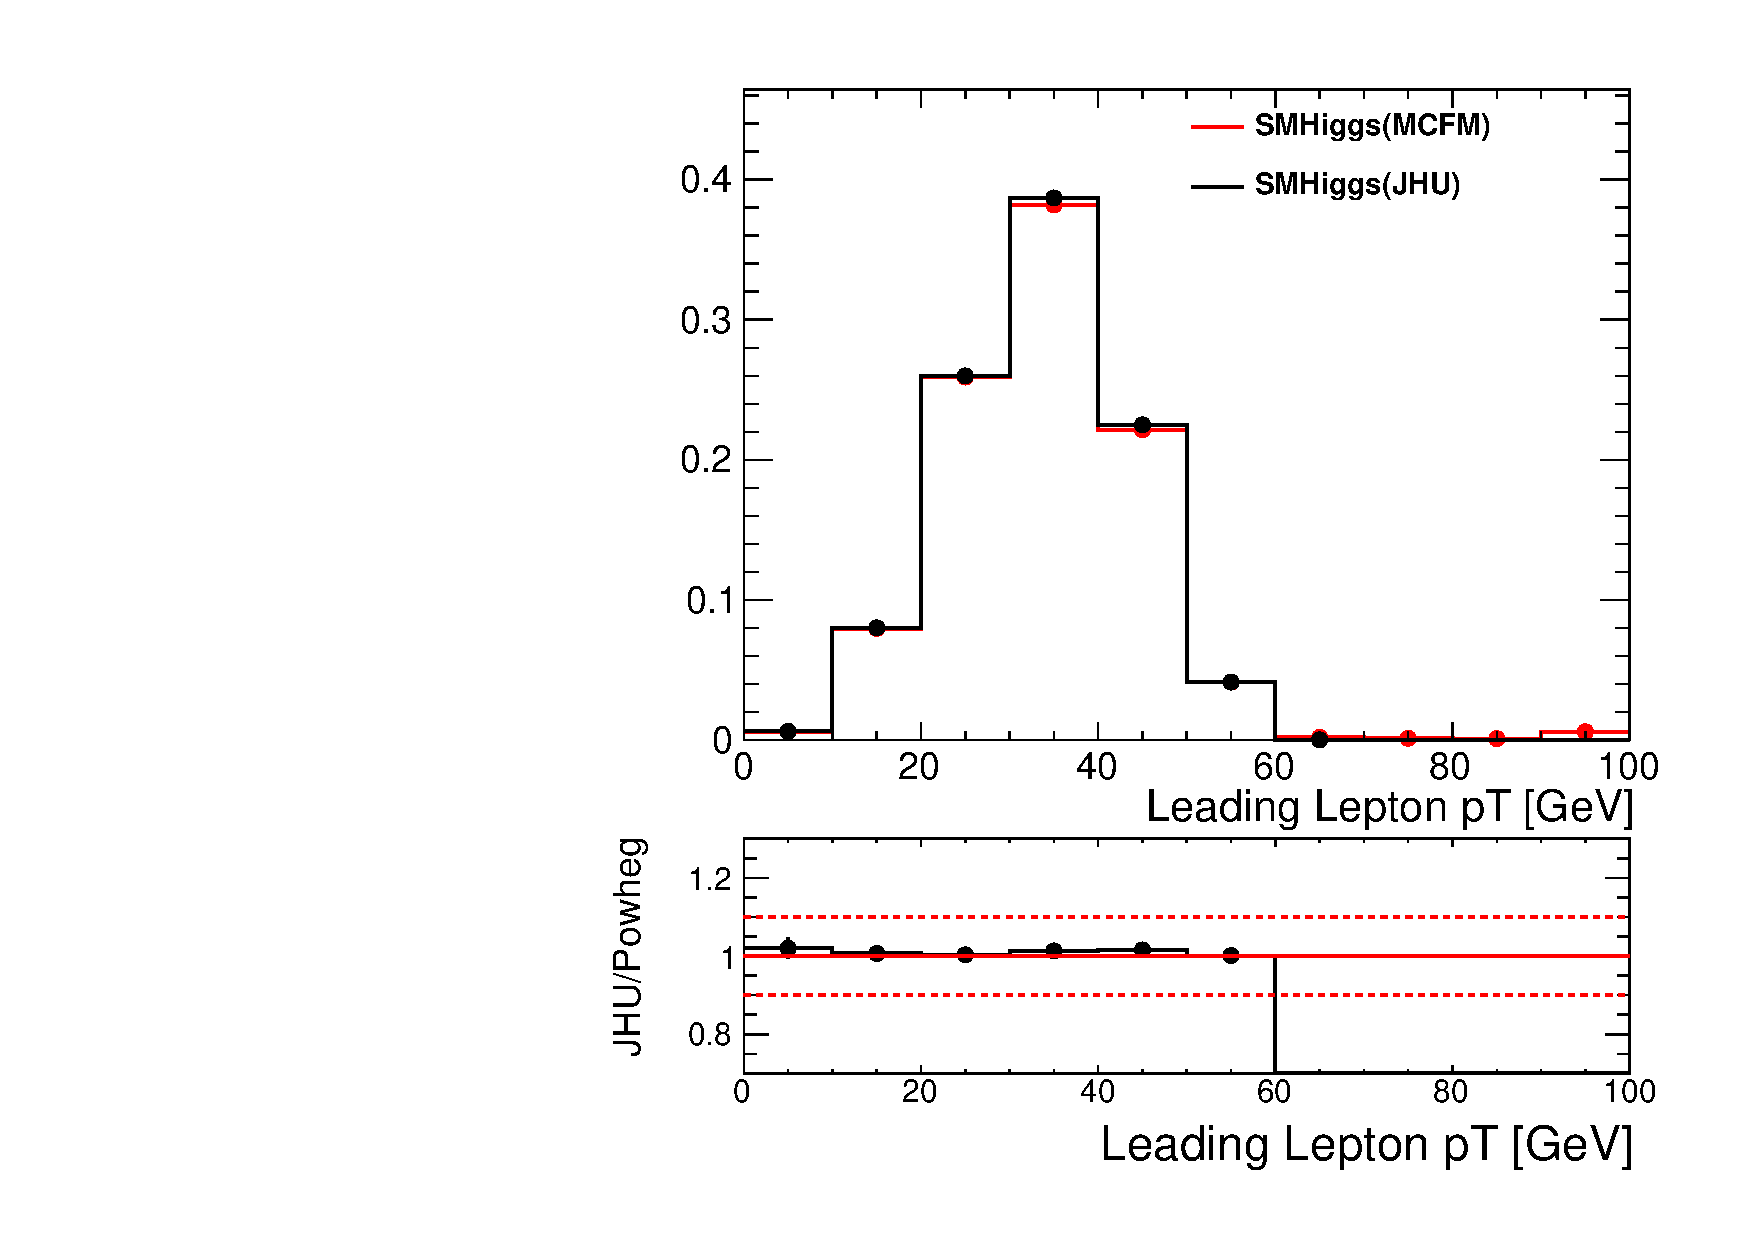
\includegraphics[width=.3\textwidth]{figures/leadleppt_jhuvsmcfm.pdf}
}
\subfigure[Trailing Lepton $p_T$]{
\centering
\label{subfig:trailleppt}
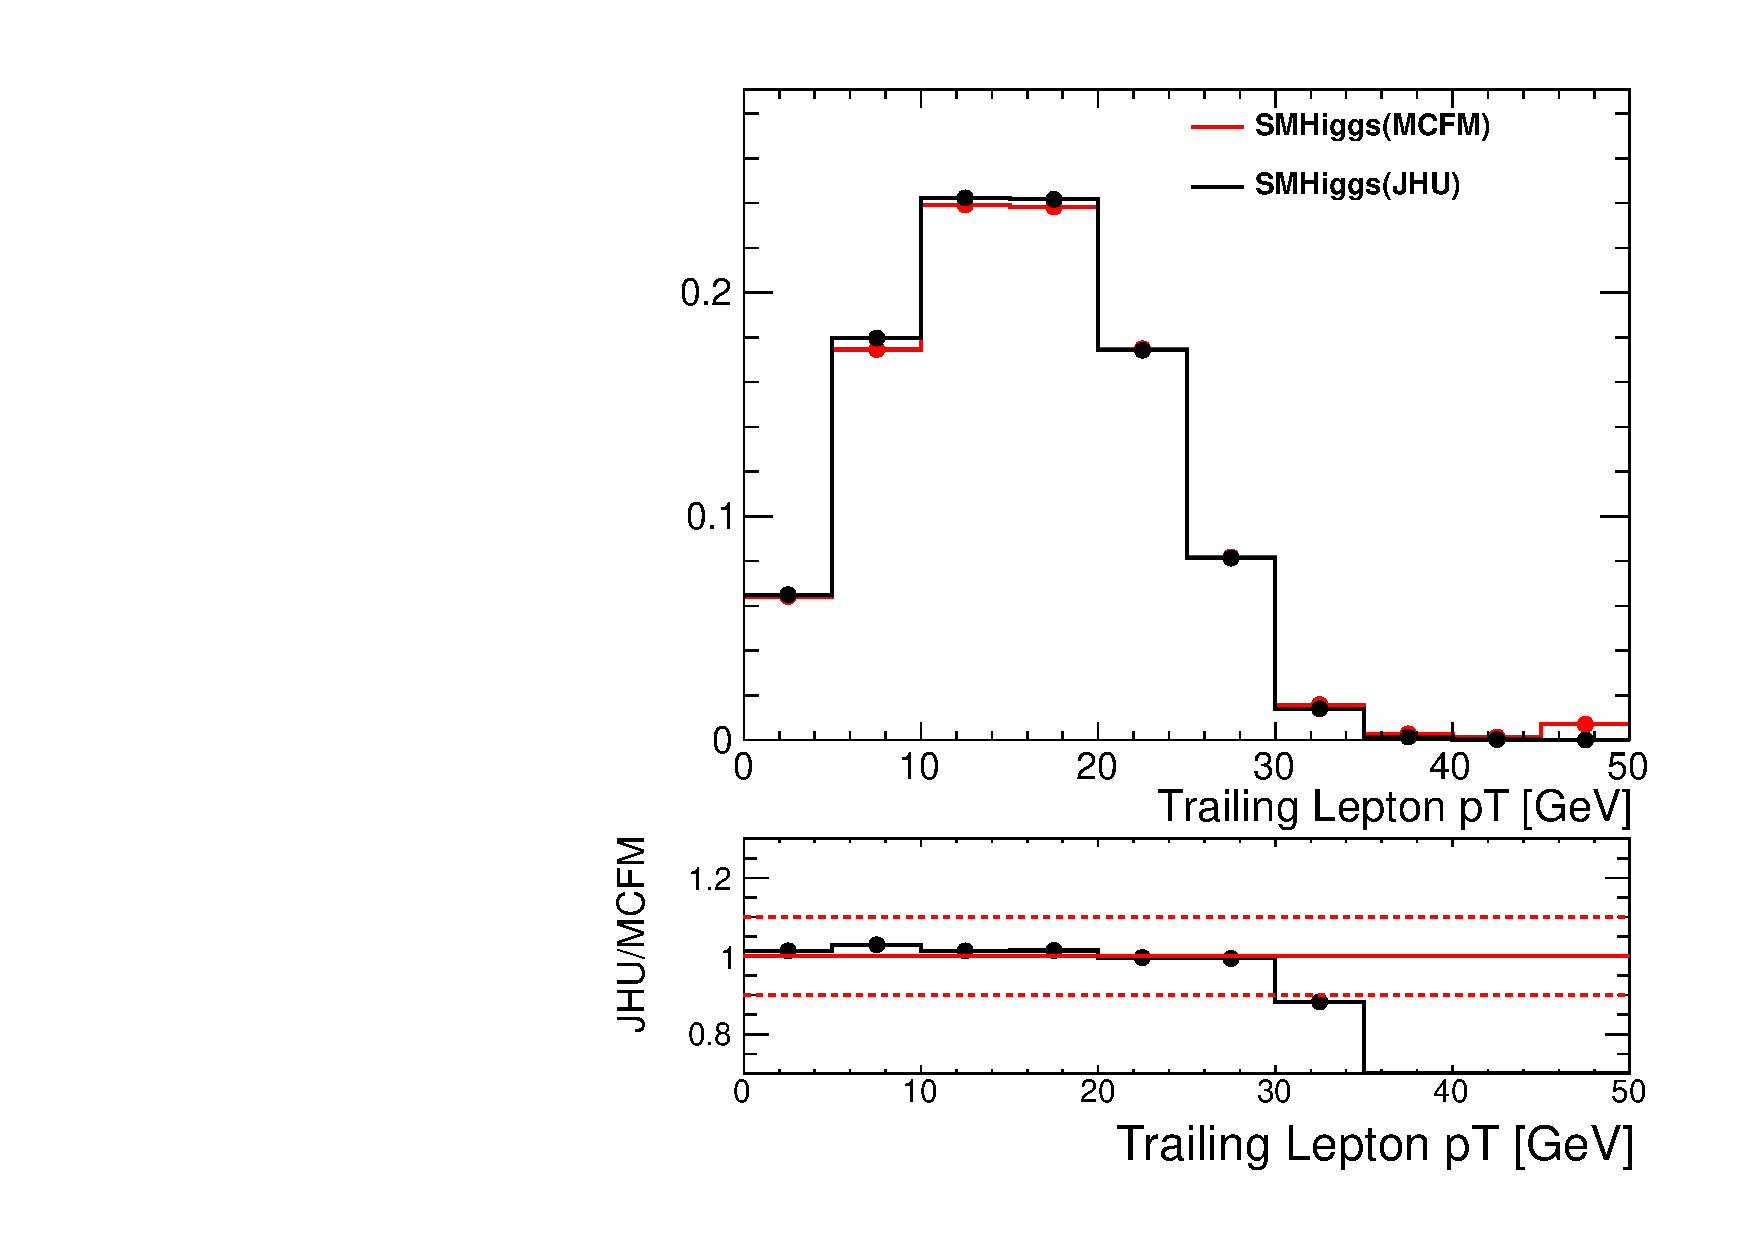
\includegraphics[width=.3\textwidth]{figures/trailleppt_jhuvsmcfm.pdf}
}
\subfigure[Leading Lepton $\eta$]{
\centering
\label{subfig:leadlepeta}
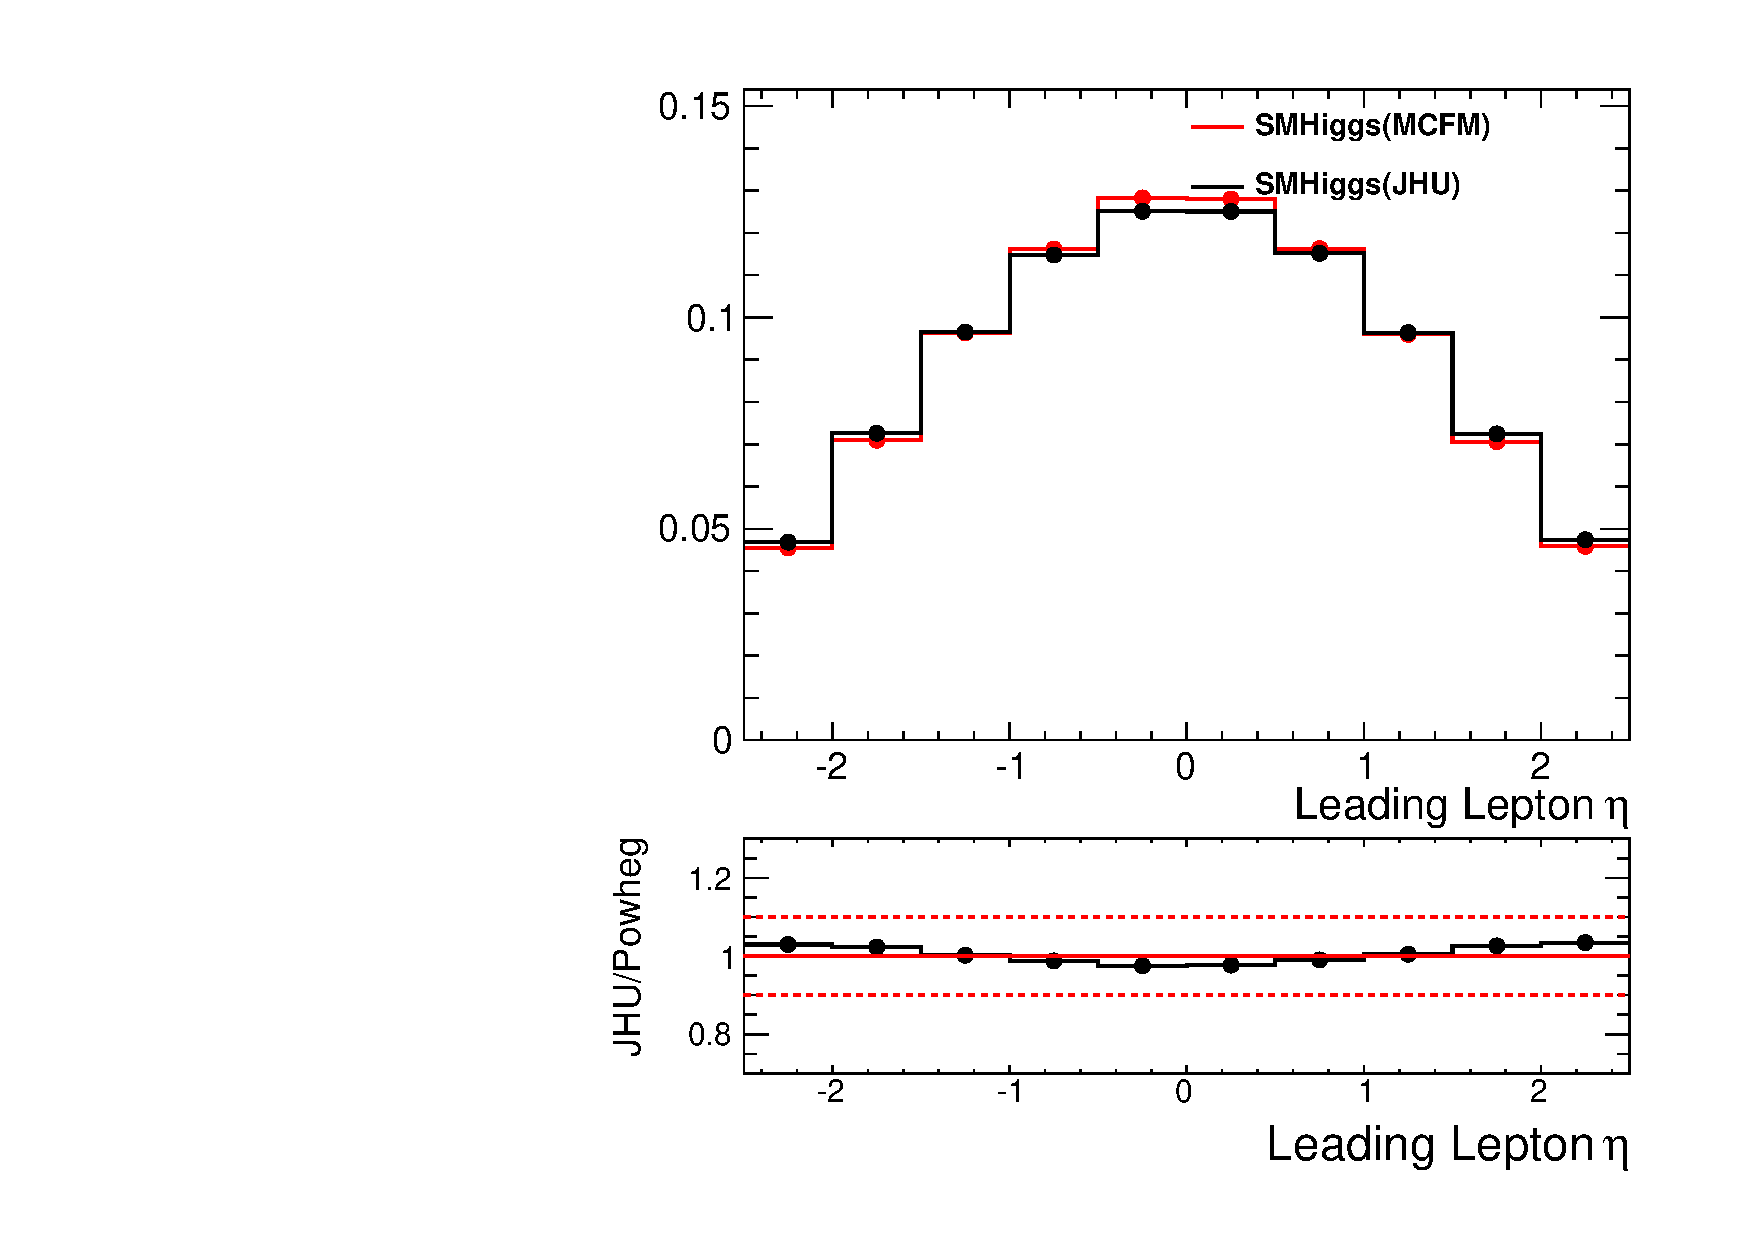
\includegraphics[width=.3\textwidth]{figures/leadlepeta_jhuvsmcfm.pdf}
} \\
\subfigure[Trailing Lepton $\eta$]{
\centering
\label{subfig:traillepeta}
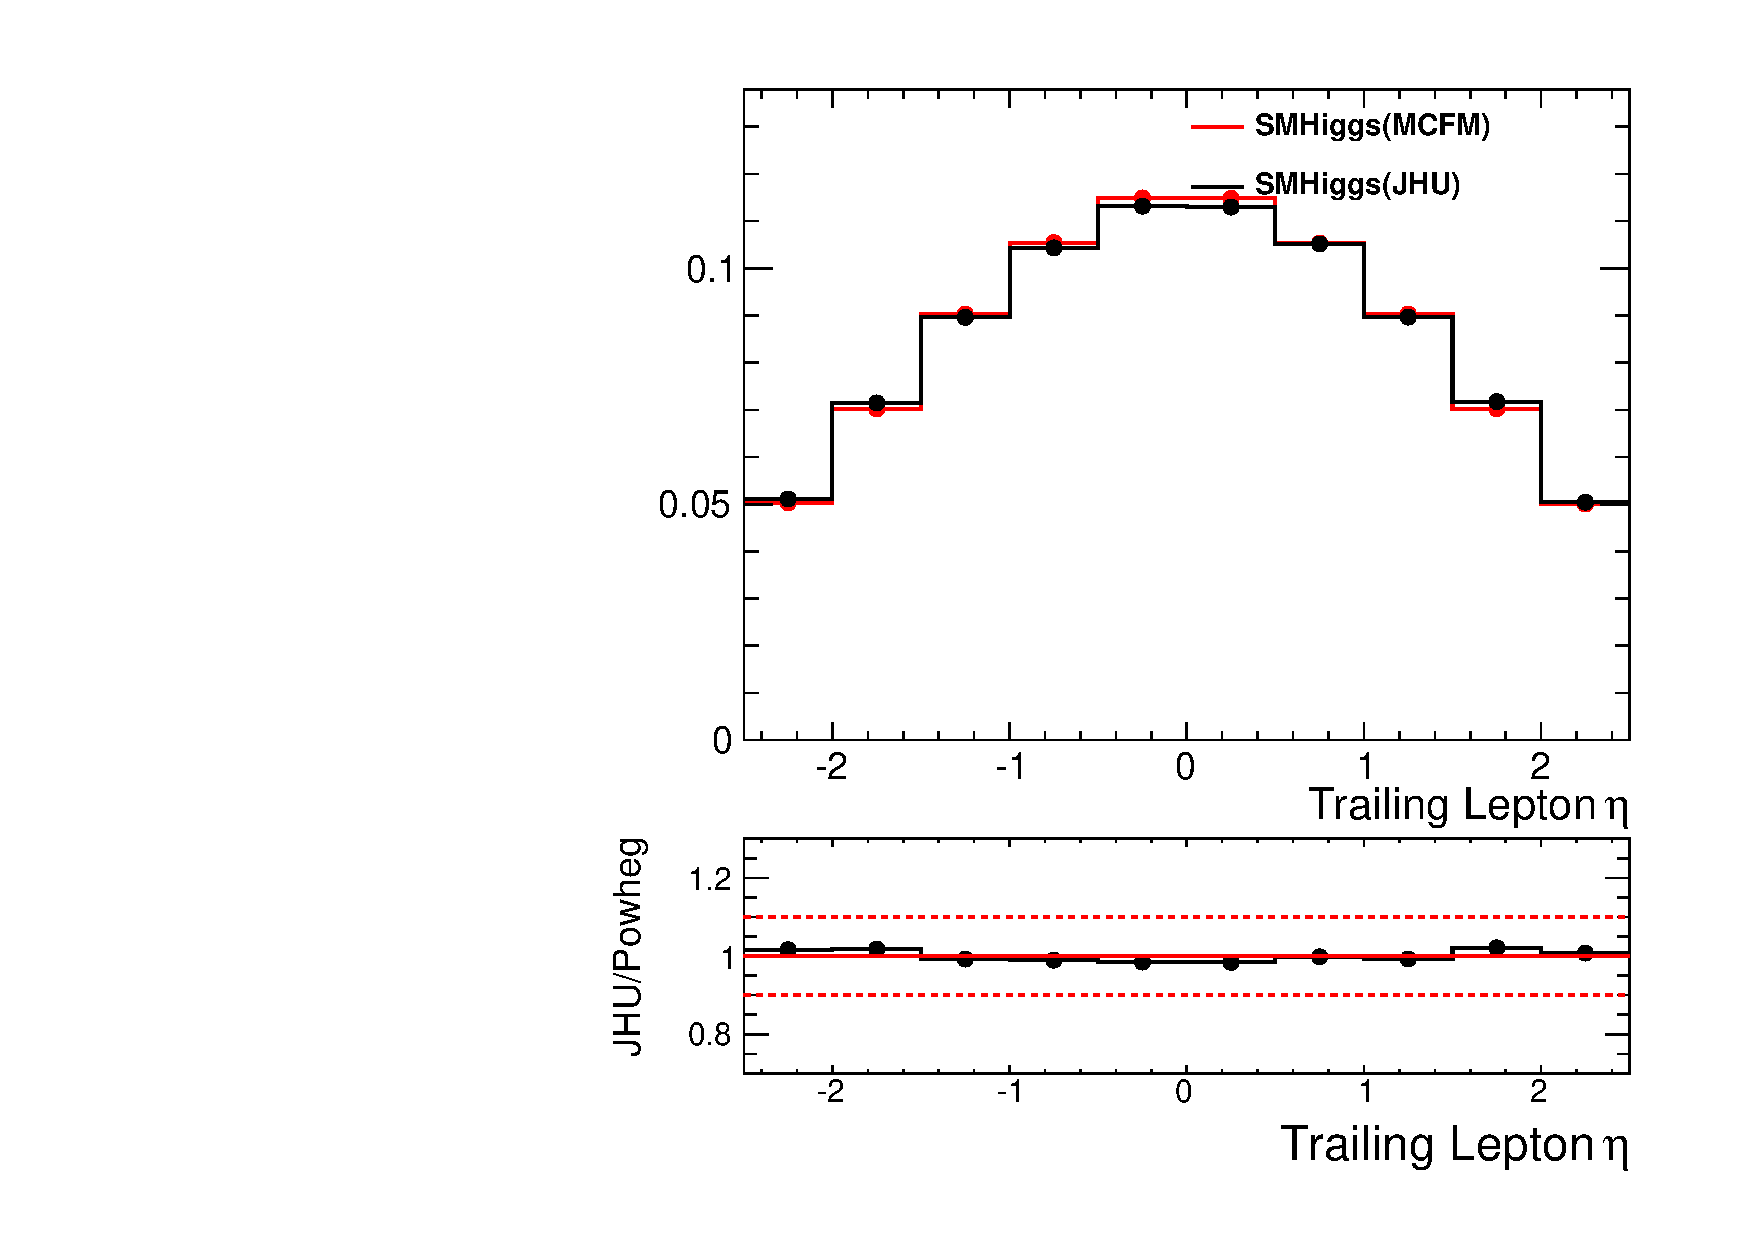
\includegraphics[width=.3\textwidth]{figures/traillepeta_jhuvsmcfm.pdf}
}
\subfigure[Dilepton mass]{
\centering
\label{subfig:mll}
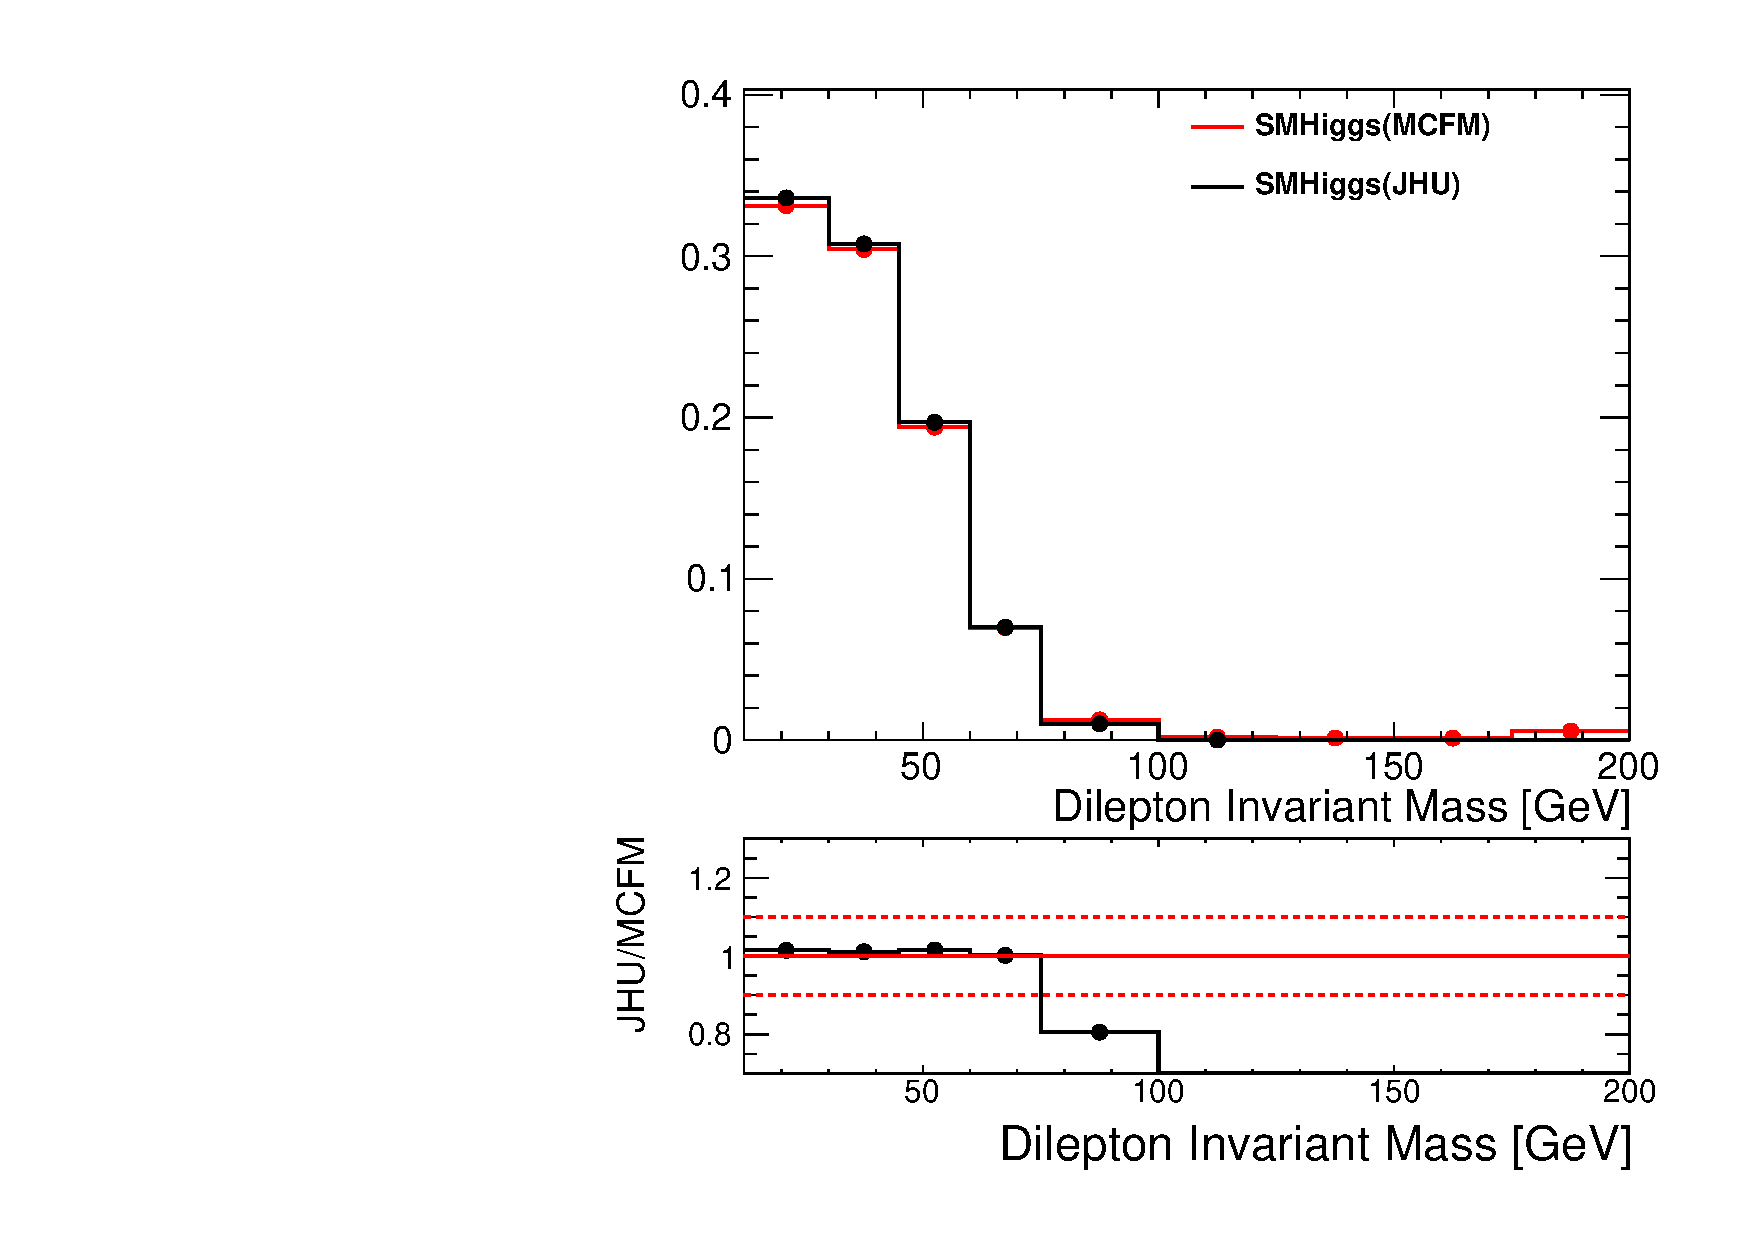
\includegraphics[width=.3\textwidth]{figures/mll_jhuvsmcfm.pdf}
} 
\subfigure[Transverse Higgs Mass]{
\centering
\label{subfig:mt}
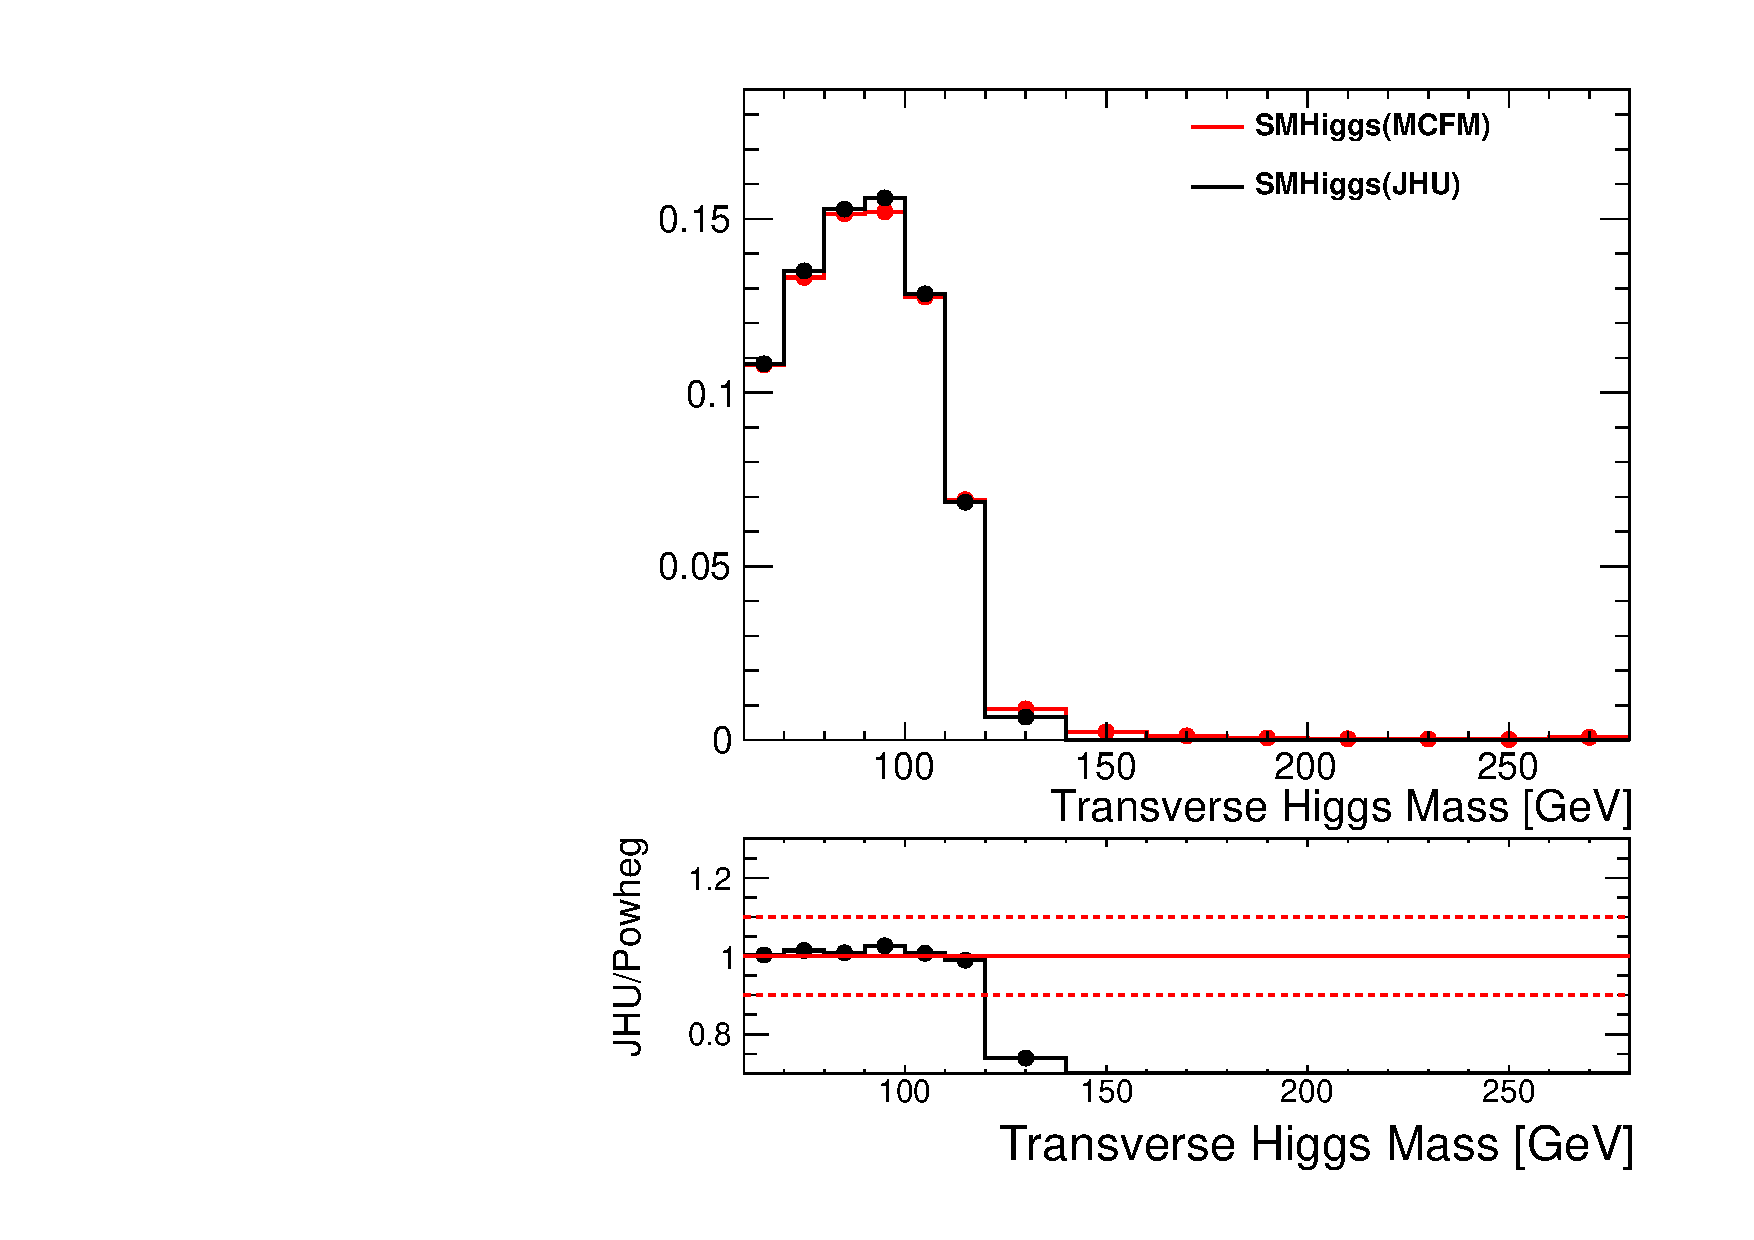
\includegraphics[width=.3\textwidth]{figures/mt_jhuvsmcfm.pdf}
}\\
\subfigure[Dilepton $p_T$]{
\centering
\label{subfig:dilpt}
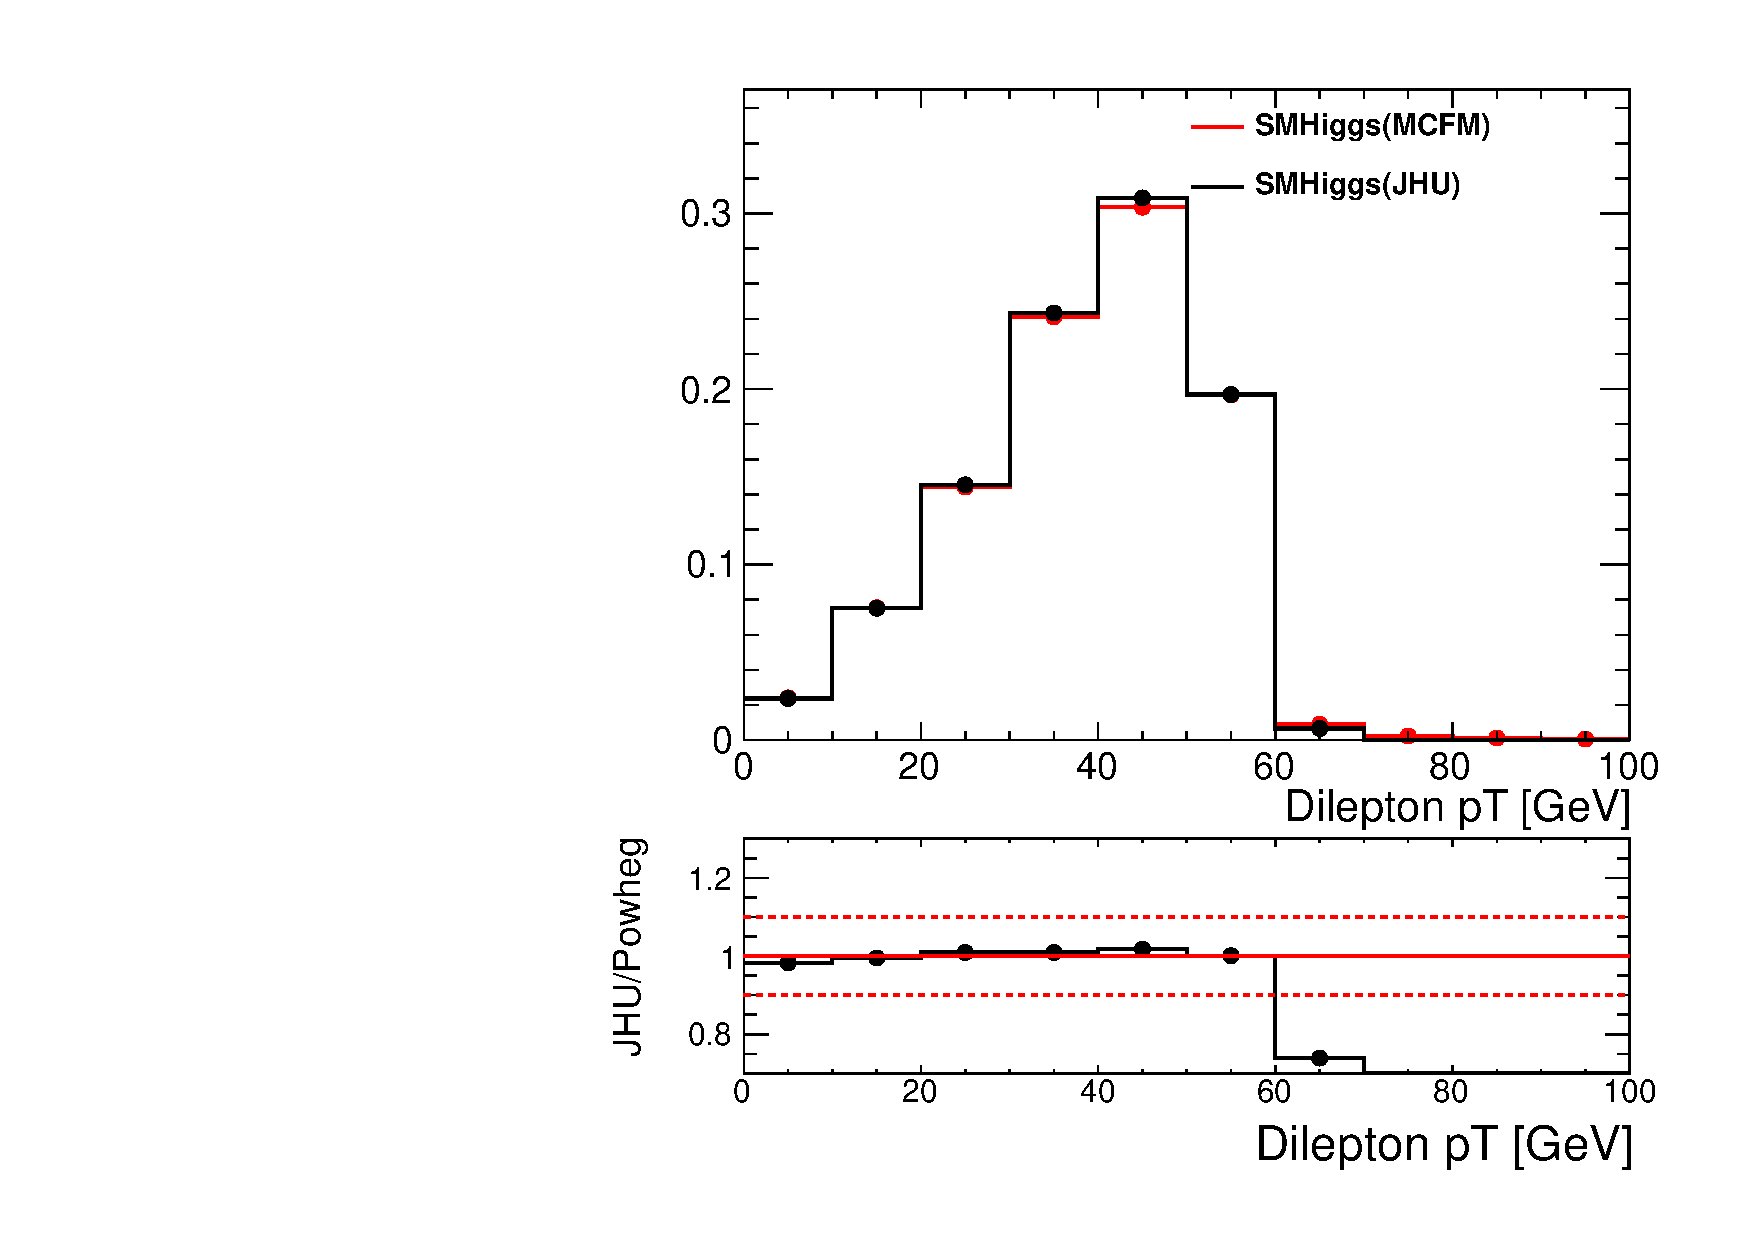
\includegraphics[width=.3\textwidth]{figures/dilpt_jhuvsmcfm.pdf}
}
\subfigure[Neutrino $p_T$]{
\centering
\label{subfig:met}
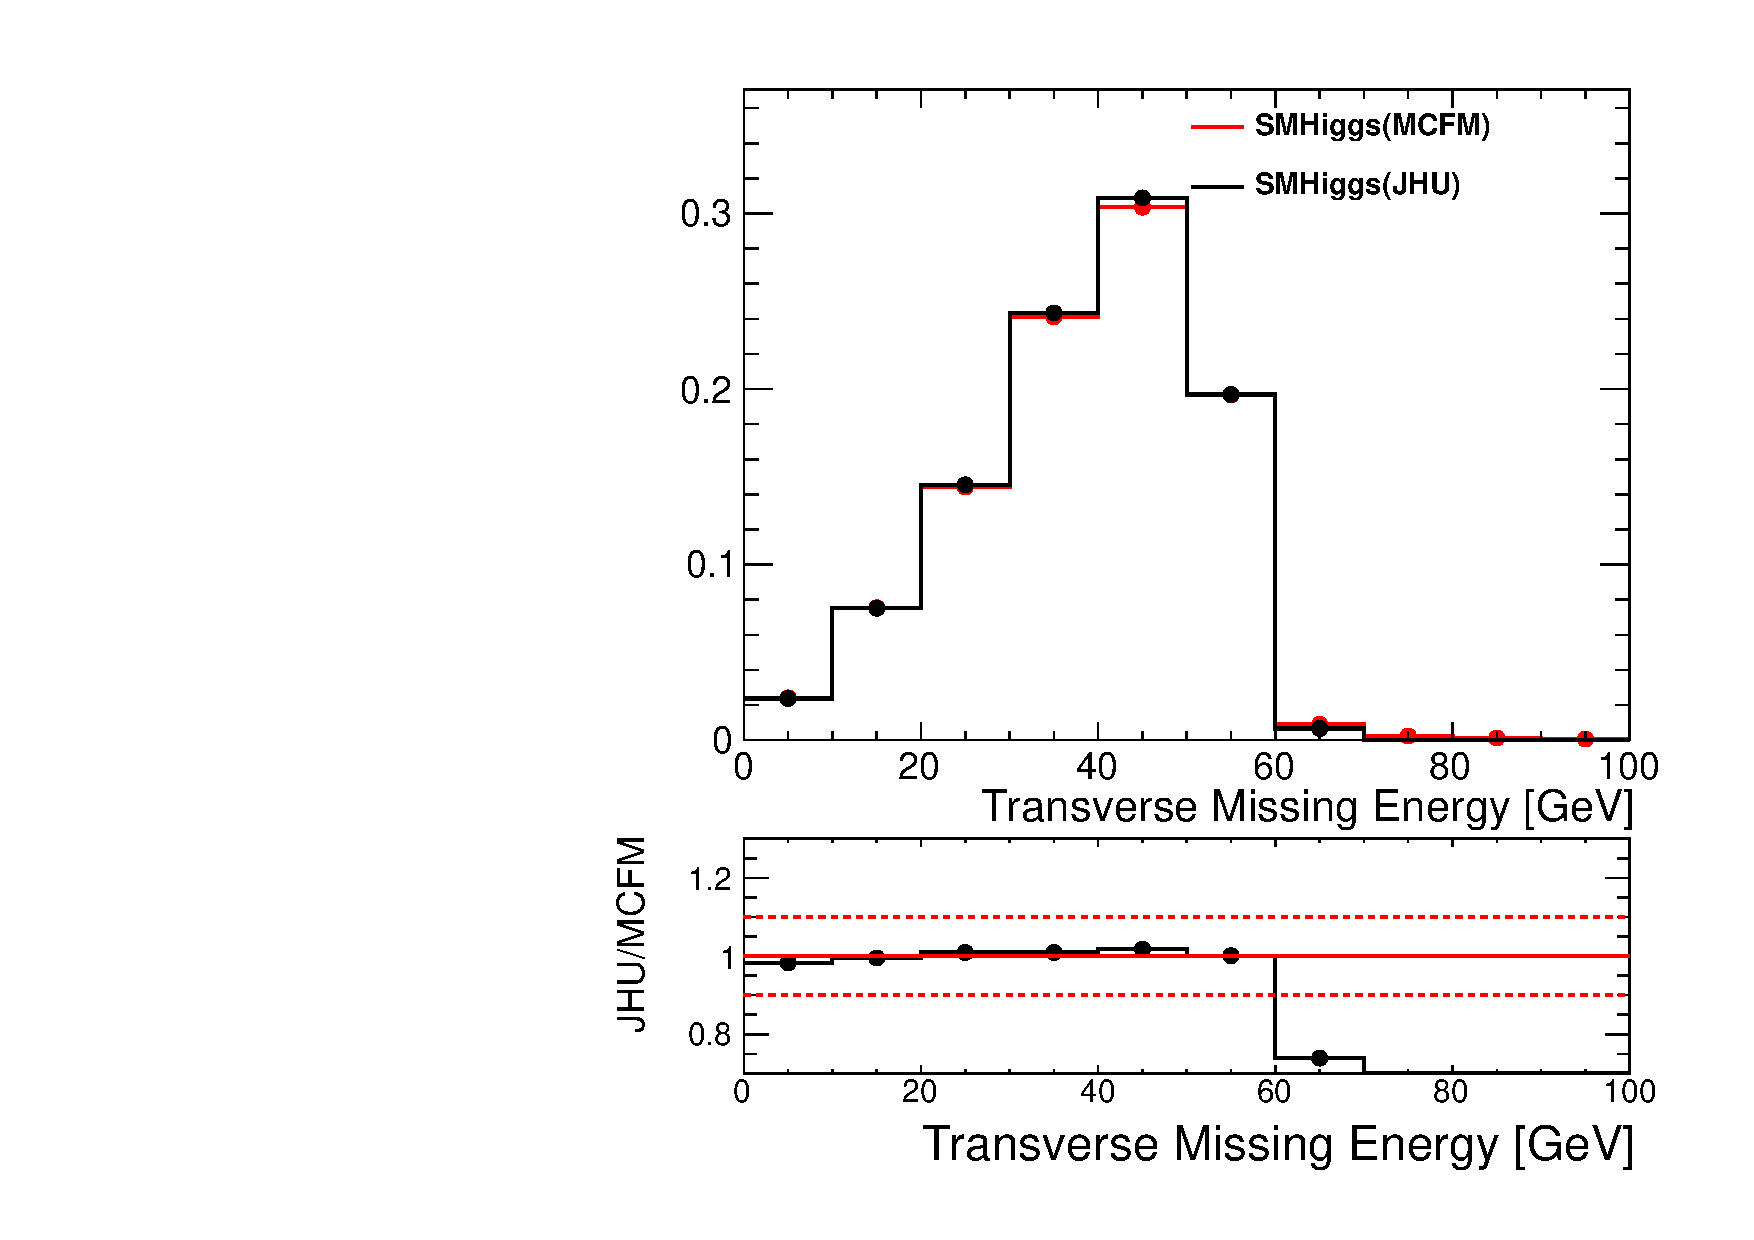
\includegraphics[width=.3\textwidth]{figures/met_jhuvsmcfm.pdf}
}
\subfigure[$\Delta\phi_{\ell\ell}$]{
\centering
\label{subfig:met}
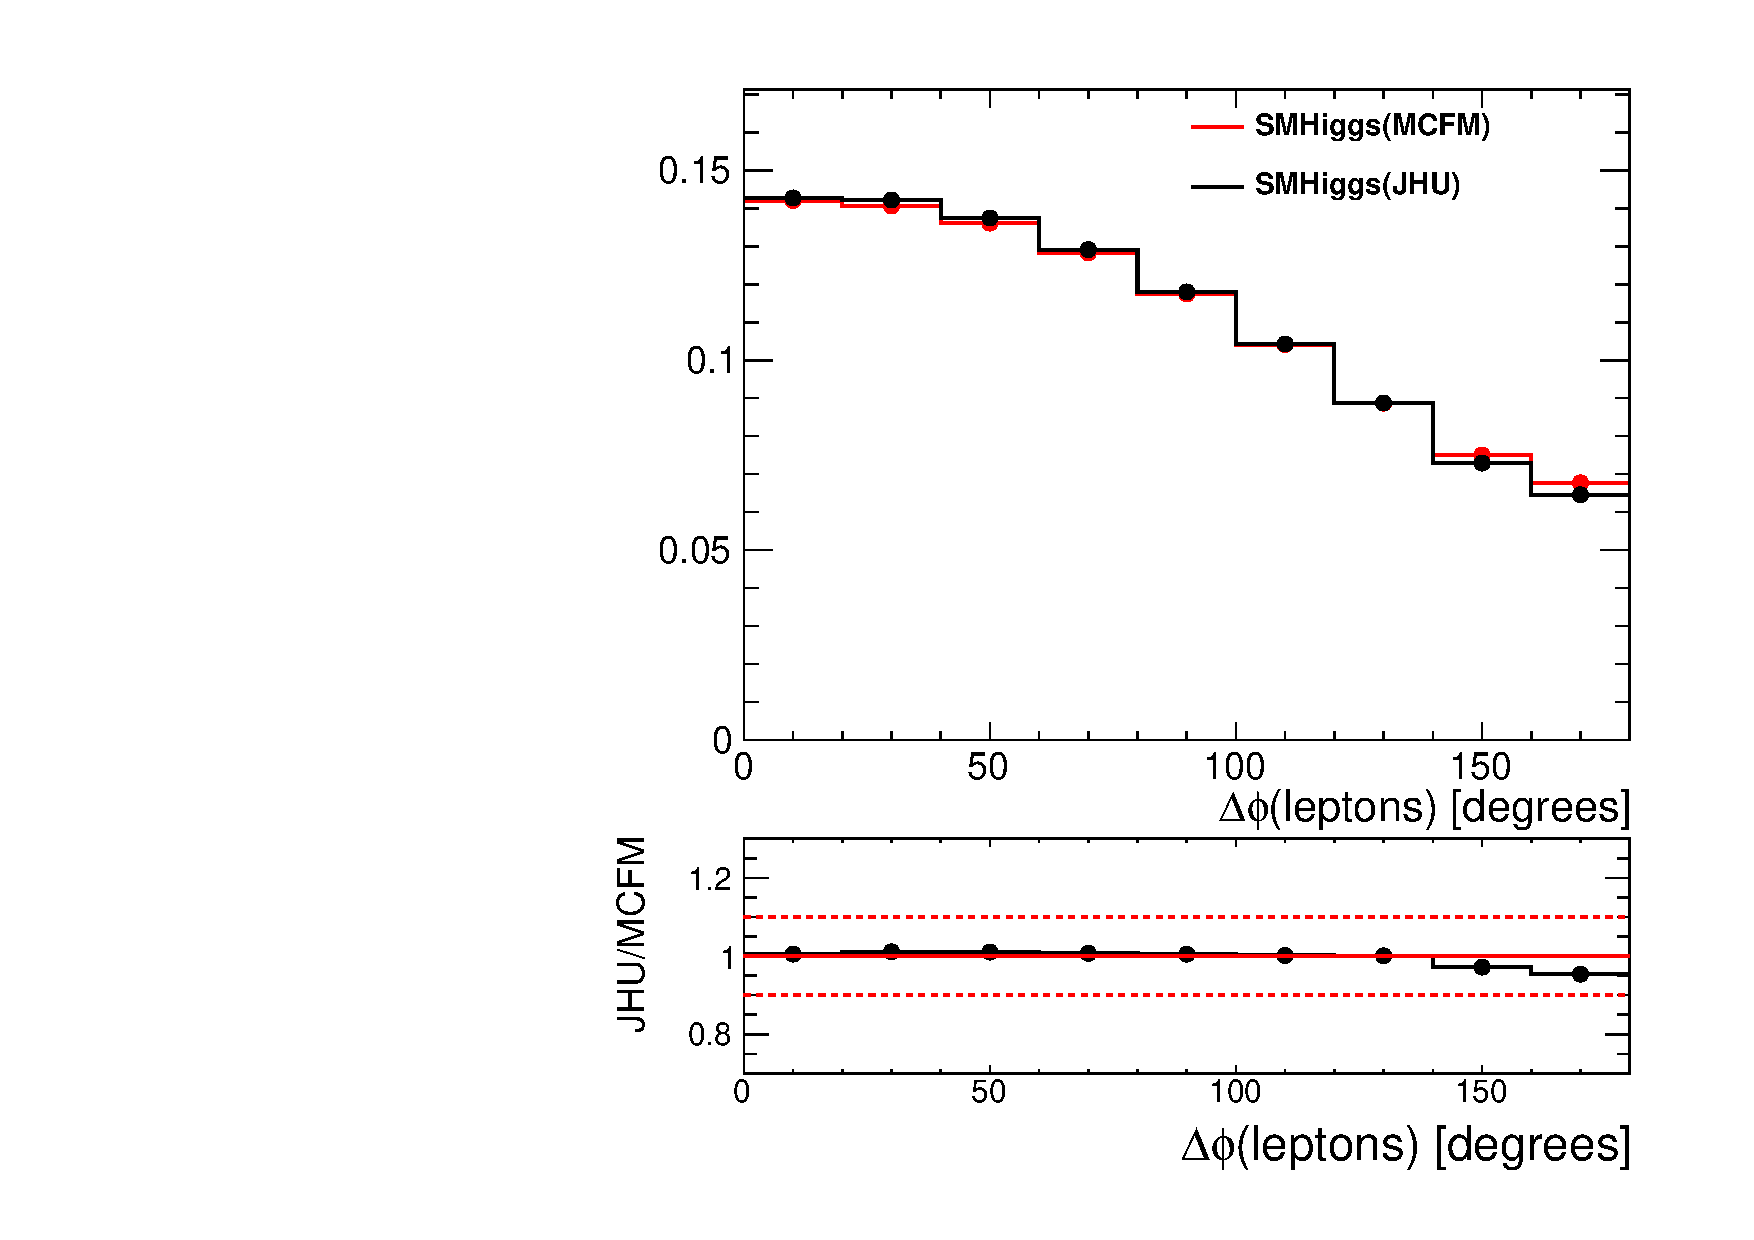
\includegraphics[width=.3\textwidth]{figures/dphill_jhuvsmcfm.pdf}
}\\
\caption{Gerator level kinematic distributions (normalized to 1) of SM Higgs 
comparing JHUGen and MCFM without any cuts. Both samples are generated with 
the Higgs produced at rest. }
\label{fig:jhuvsmcfm}
\end{figure}
%%%%%%%%%%%%%%%%%%%%%%%%%%%%%%%%%%%%%%%%%%%%%

Figure~\ref{fig:higgspt_0j} shows the Higgs $p_T$ and the leading jet 
$p_T$ distributions for the SM Higgs hypothesis comparing the 
JHUGen-Pythia and Powheg-Pythia~\cite{powheg} samples, after applying the full 
event selections. The two generators agree within 10\%. 
The differences are expected as the Powheg sample is generated with the 
NLO calculations at the matrix element level. 
The effects on the main kinematic observables due to 
the difference in Higgs $p_T$ however are smaller, shown in Figure~\ref{fig:higgskin_0j}. 

To account for the missing higher order effects we reweight 
the SM Higgs templates in the final analysis 
to match to the predictions by Powheg-Pythia. 
The relative differences between JHUGen and Powheg in the SM Higgs are then 
applied to the other signal hypothesis as well assuming the same effects mainly 
because all resonances are colorless objects. 
%Therefore the missing higher 
%order effects are similar between different hypotheses. 
Figure~\ref{fig:gravvshiggspt_0j} shows the resonance $p_T$ and 
the leading jet $p_T$ distributions comparing the spin 2 
graviton and the SM Higgs hypothesis generated with the JHUGen-Pythia. 
The two hypotheses agree within a few \% in the bulk of the distributions, 
smaller than the differences between Powheg-Pythia and JHUGen-Pythia 
in the SM Higgs hypothesis. 
Additional shape systematics due to this difference is then added as well, see section~\ref{sec:systematics}. 


%%%%%%%%%%%%%%%%%%%%%%%%%%%%%%%%%%%%%%%%%%%%%
\begin{figure}[!hbtp]
\centering
\subfigure[Higgs $p_T$]{
\centering
\label{subfig:higgspt_0j}
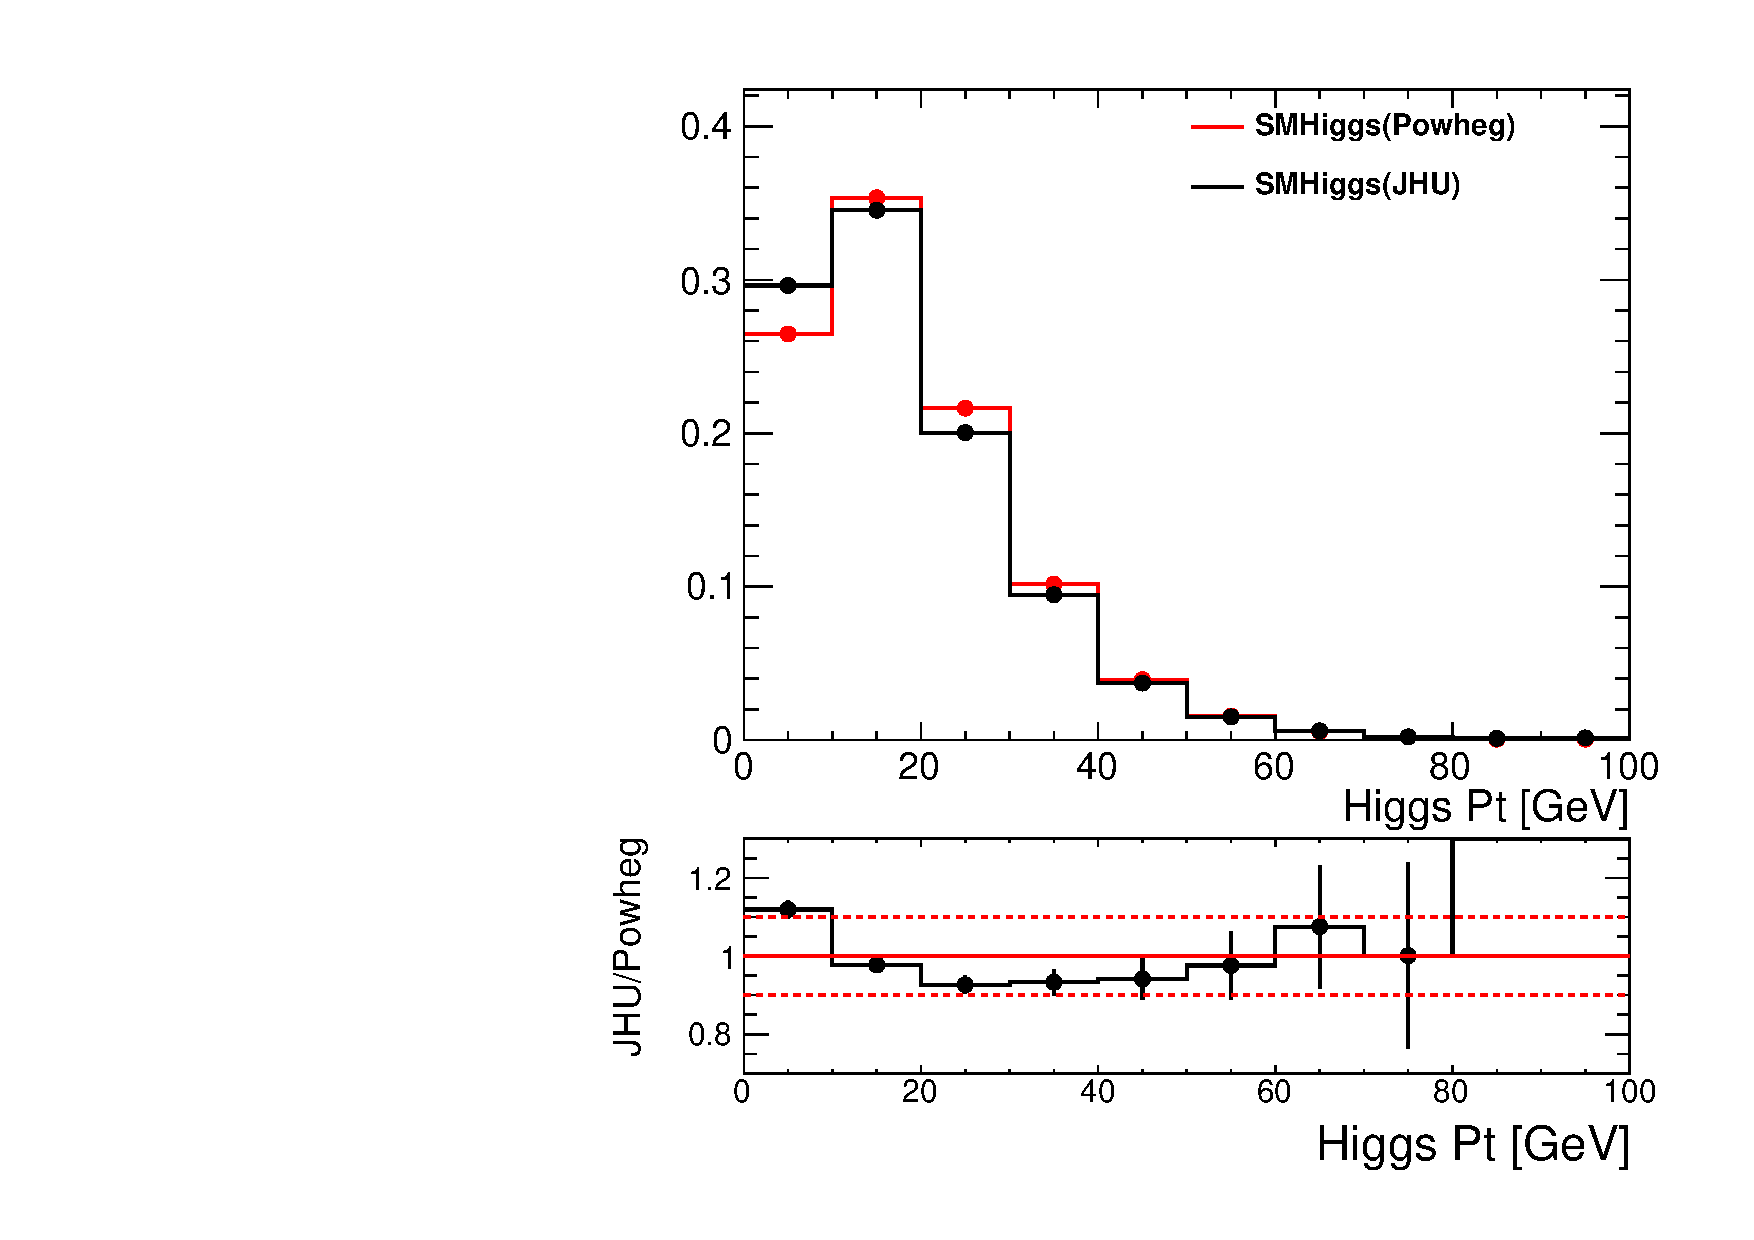
\includegraphics[width=.3\textwidth]{figures/higgsPt.pdf}
}
\subfigure[Leading Jet $p_T$]{
\centering
\label{subfig:jet1pt_0j}
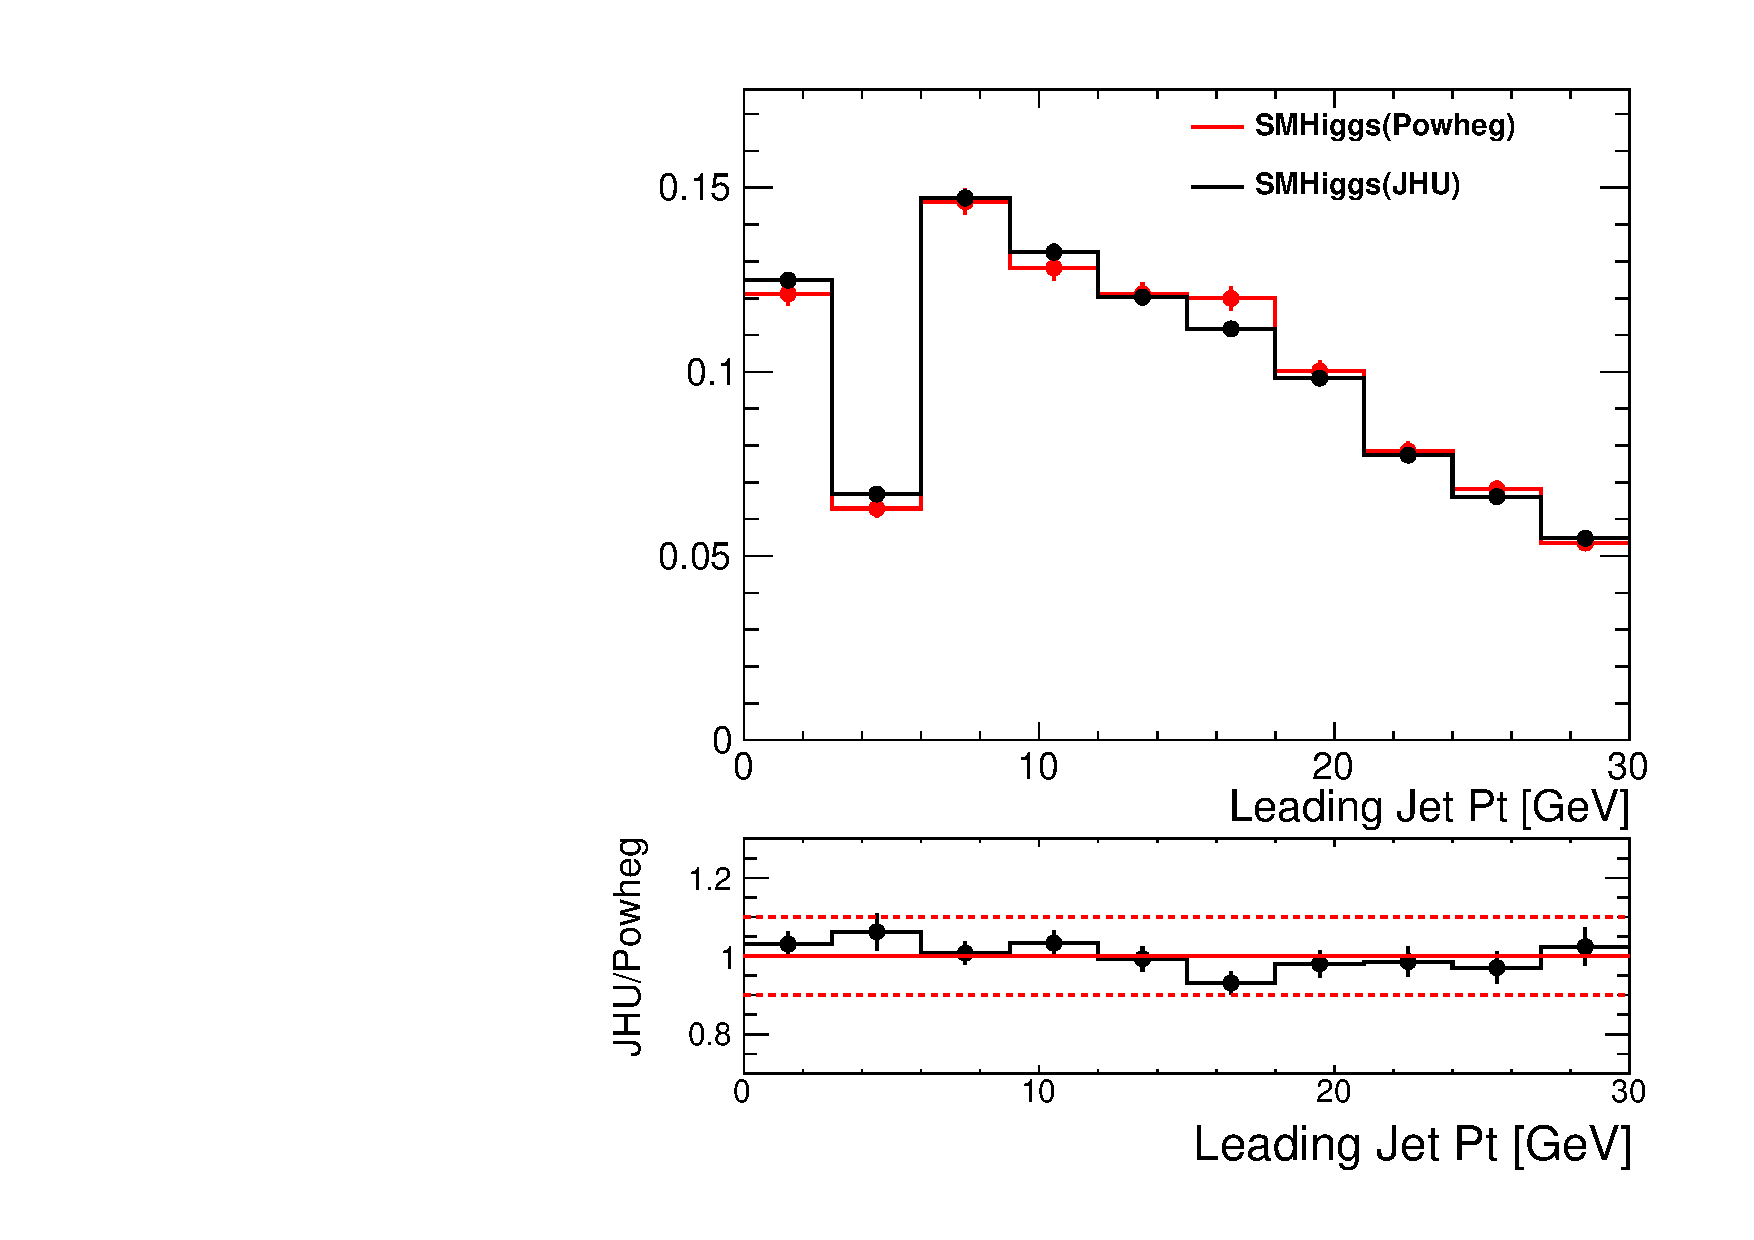
\includegraphics[width=.3\textwidth]{figures/jet1pt.pdf}
}\\
\caption{The Higgs $p_T$ and the leading jet $p_T$ distributions (normalized to 1) of the 
SM Higgs hypothesis comparing the powheg generator and JHUGen, after 
applying the final event selections. }
\label{fig:higgspt_0j}
\end{figure}
%%%%%%%%%%%%%%%%%%%%%%%%%%%%%%%%%%%%%%%%%%%%%


%%%%%%%%%%%%%%%%%%%%%%%%%%%%%%%%%%%%%%%%%%%%%
\begin{figure}[!hbtp]
\centering
\subfigure[Leading Lepton $p_T$]{
\centering
\label{subfig:leadleppt}
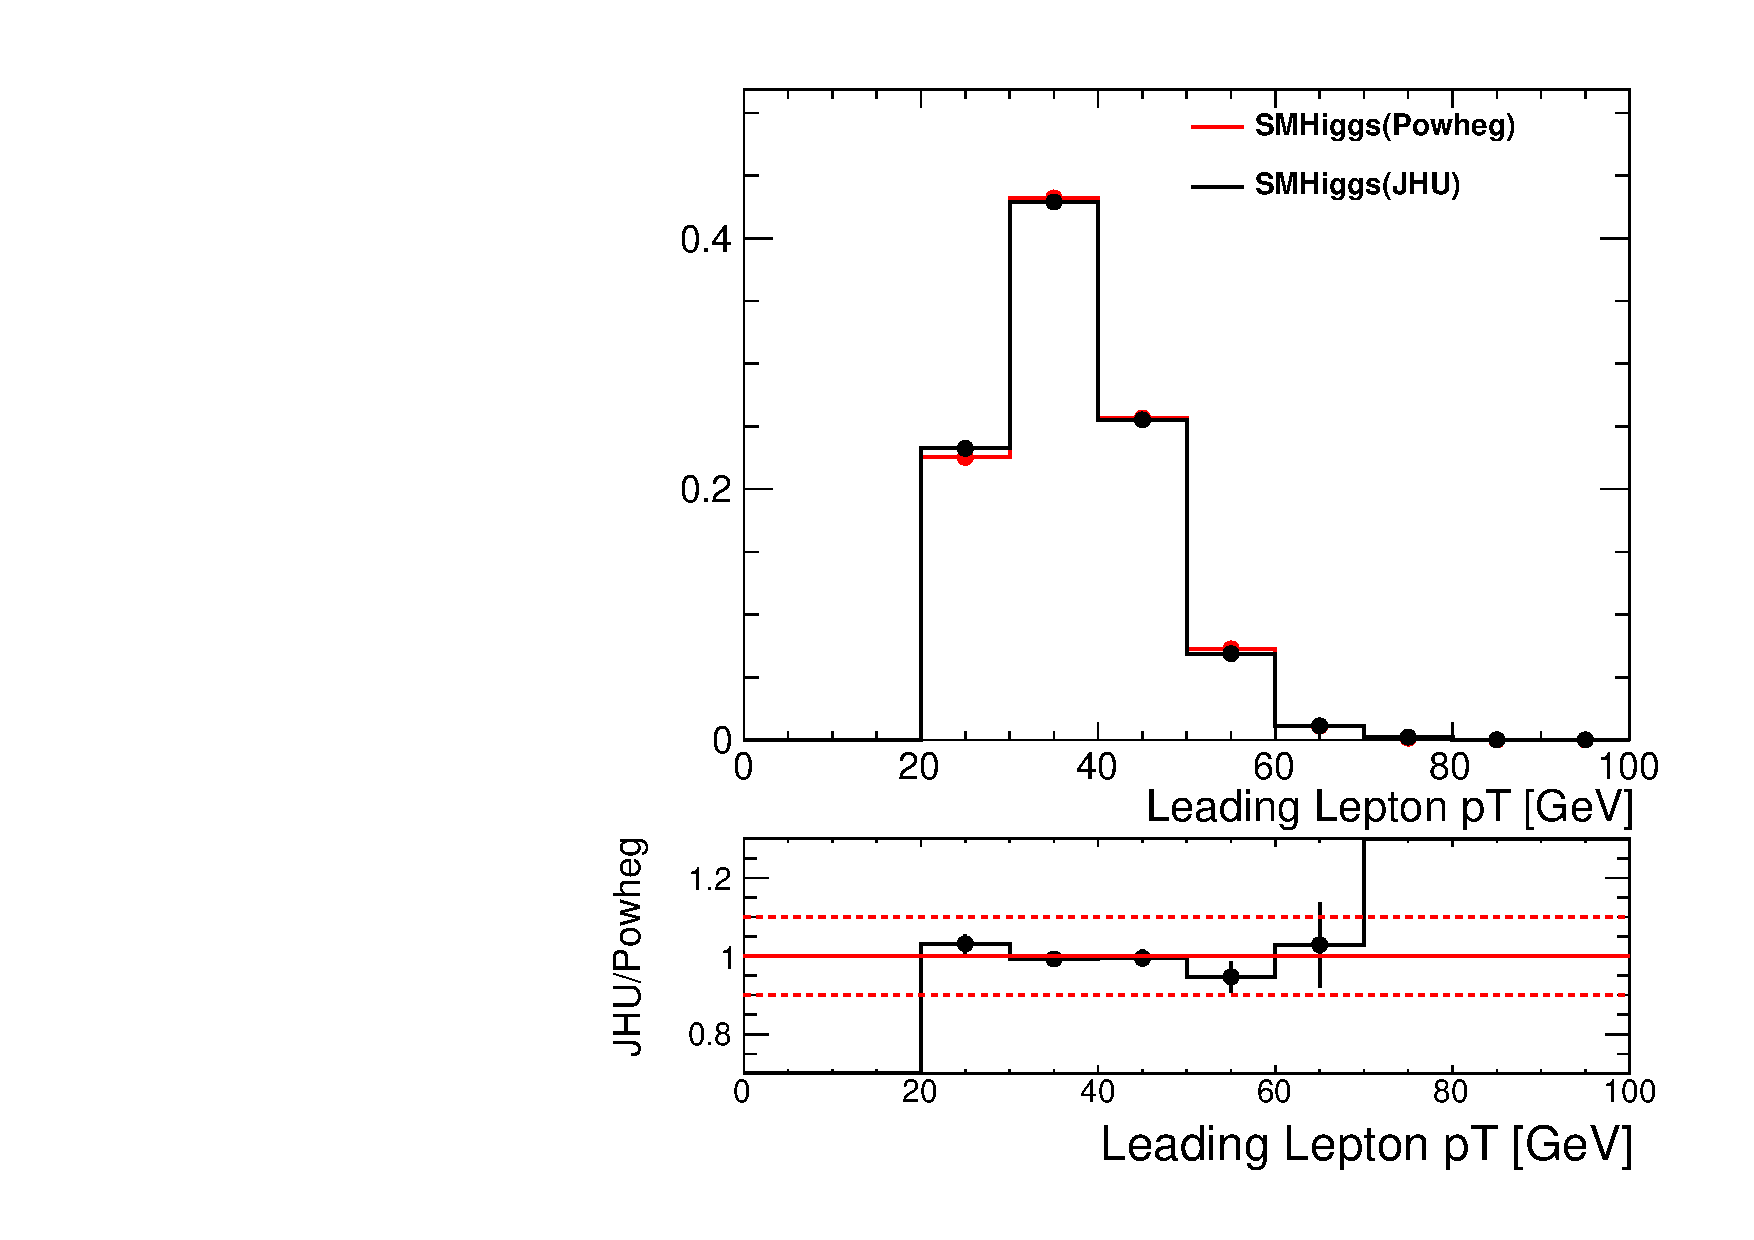
\includegraphics[width=.3\textwidth]{figures/leadleppt.pdf}
}
\subfigure[Trailing Lepton $p_T$]{
\centering
\label{subfig:trailleppt}
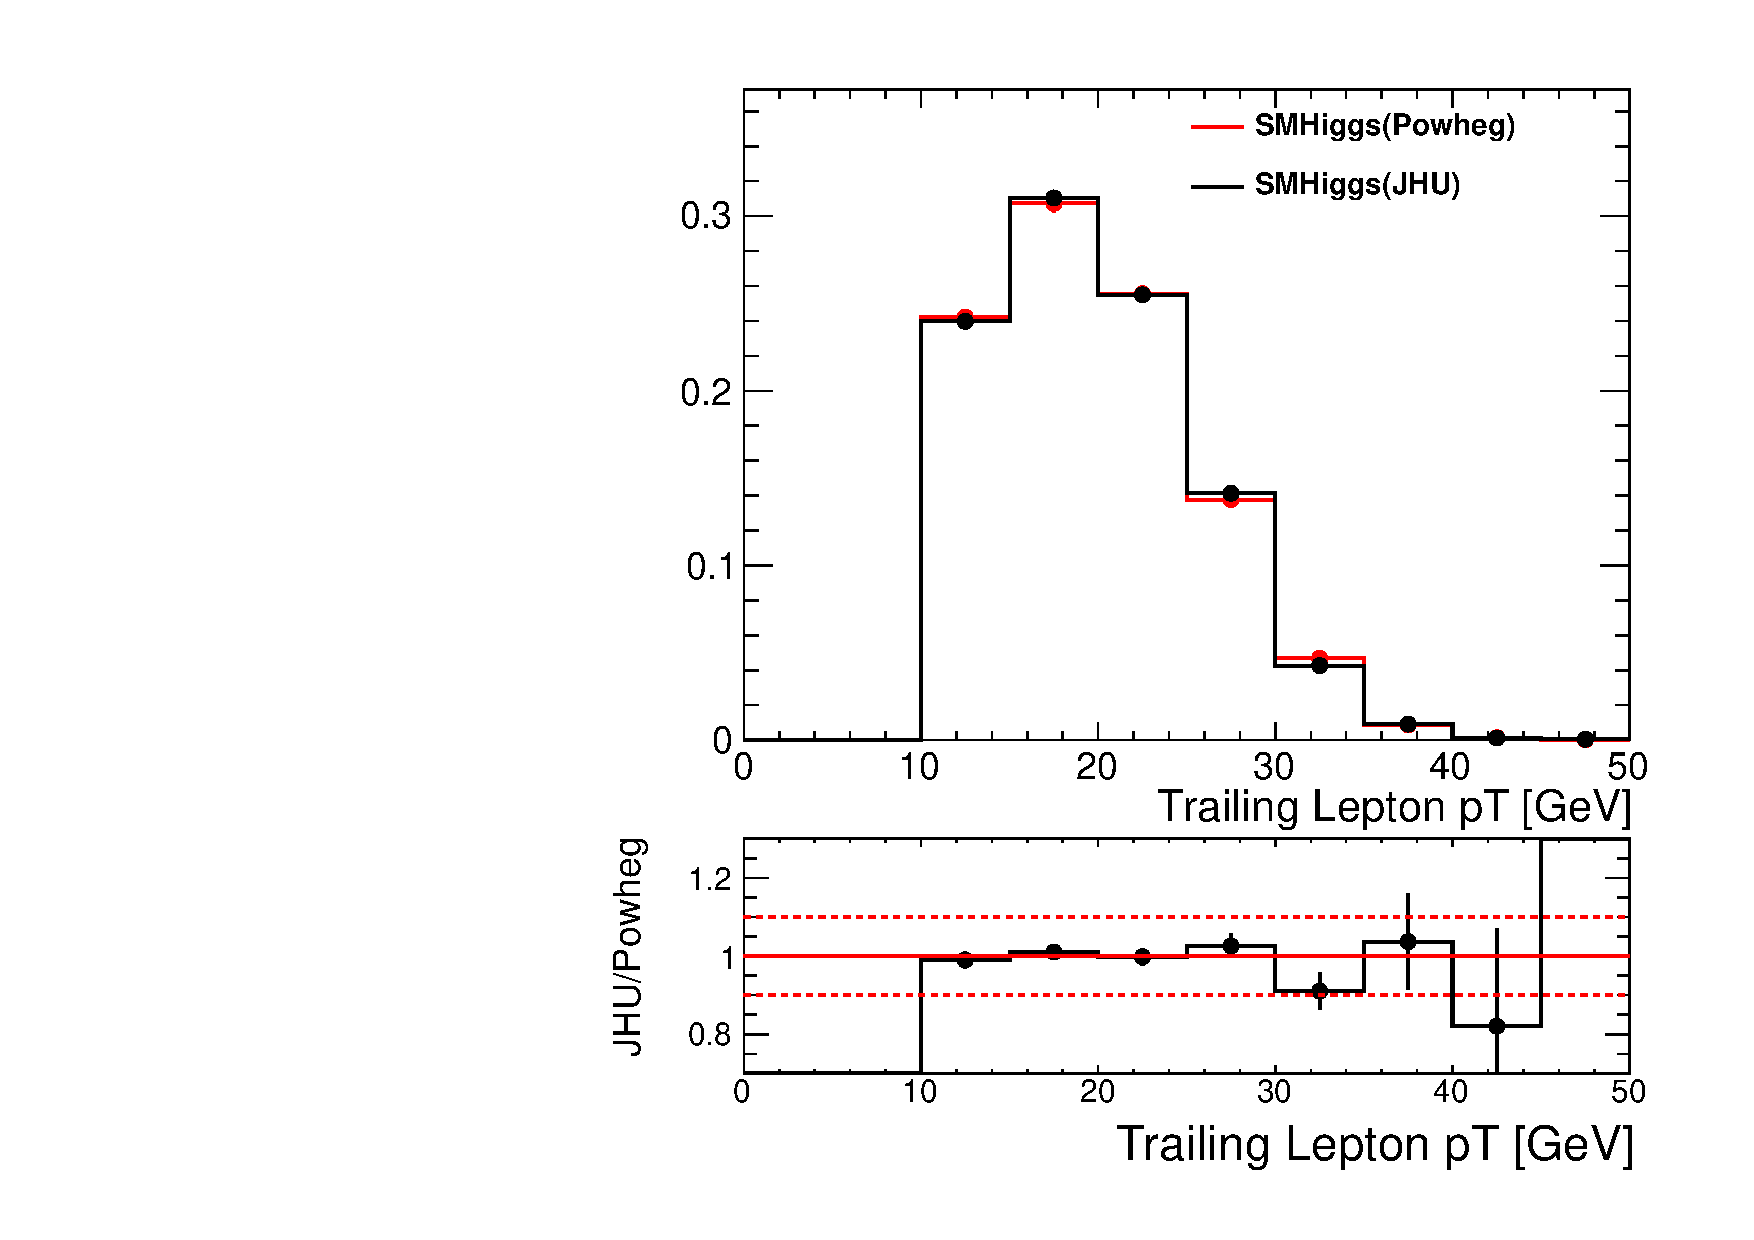
\includegraphics[width=.3\textwidth]{figures/trailleppt.pdf}
}
\subfigure[Leading Lepton $\eta$]{
\centering
\label{subfig:leadlepeta}
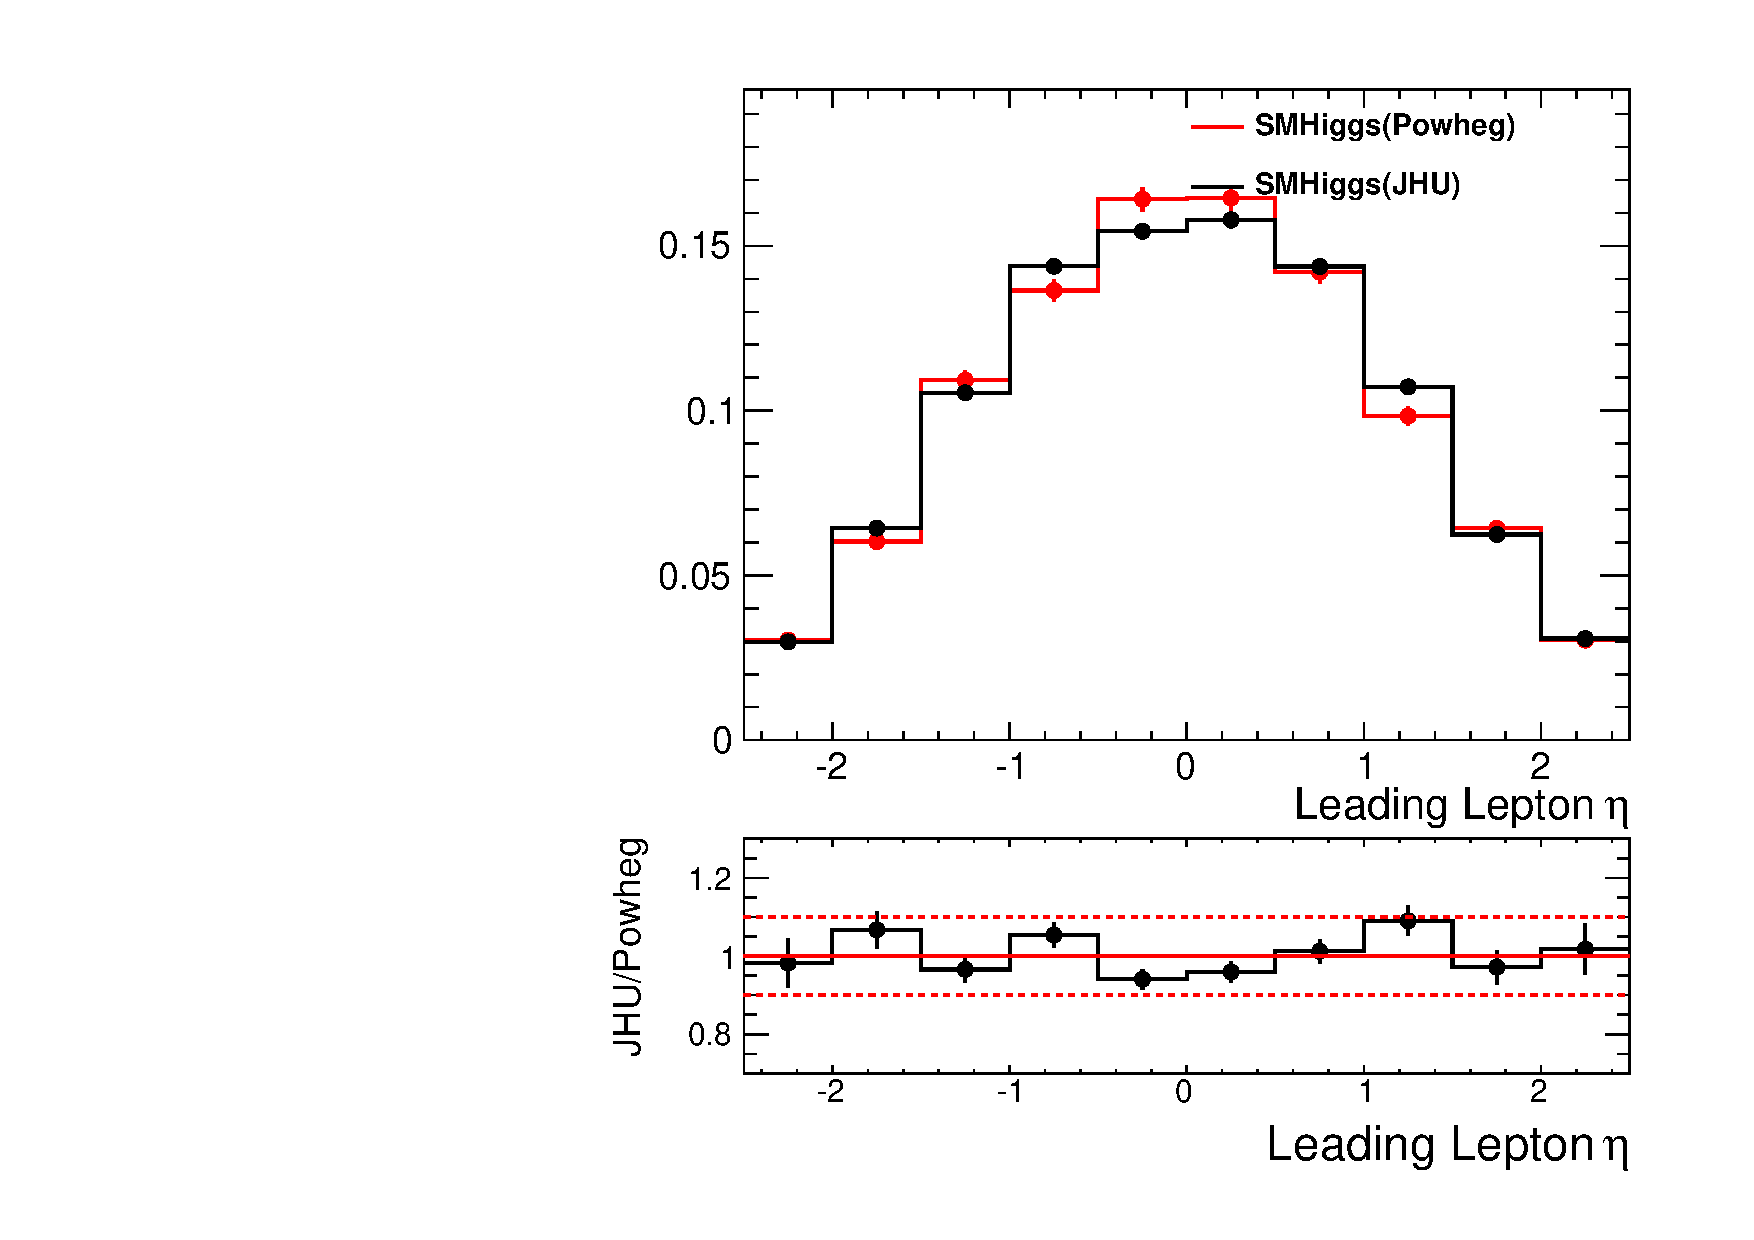
\includegraphics[width=.3\textwidth]{figures/leadlepeta.pdf}
} \\
\subfigure[Trailing Lepton $\eta$]{
\centering
\label{subfig:traillepeta}
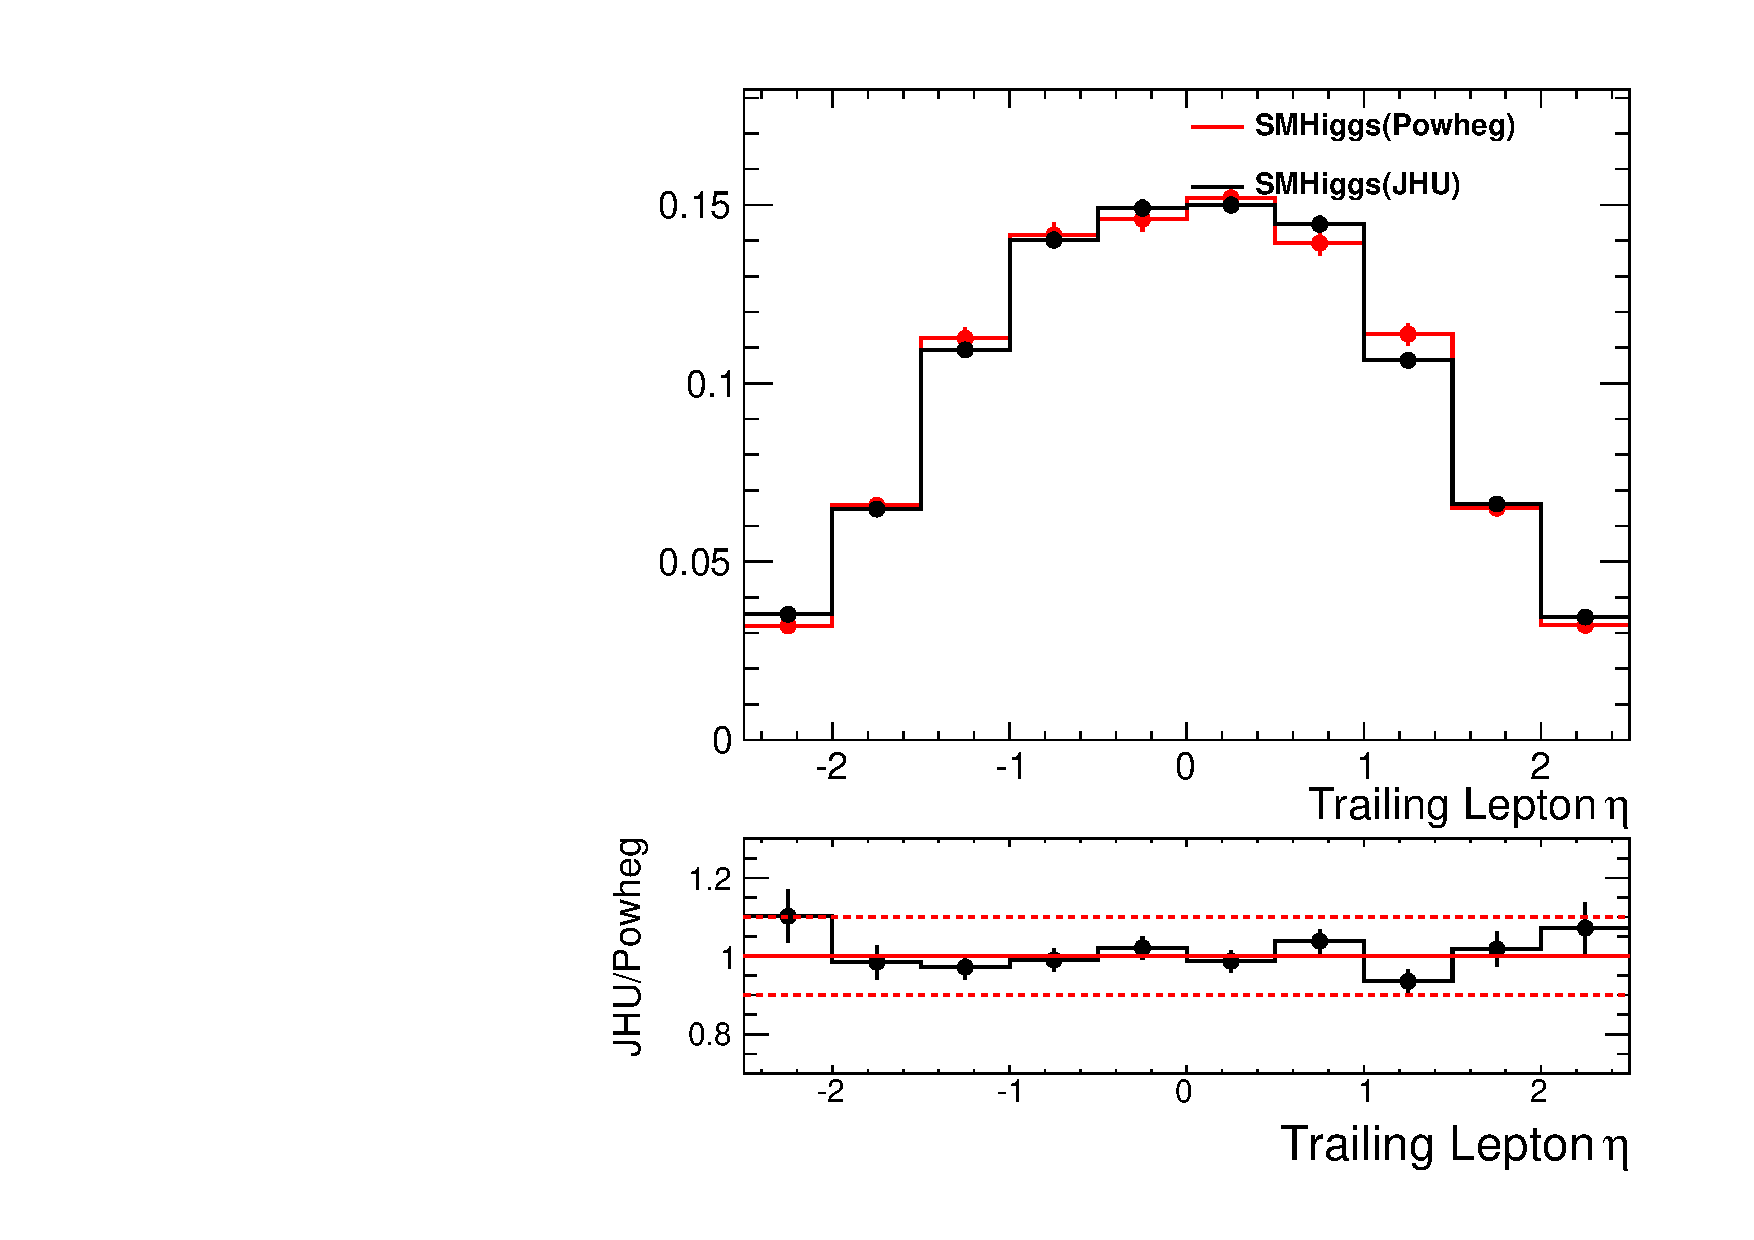
\includegraphics[width=.3\textwidth]{figures/traillepeta.pdf}
}
\subfigure[Dilepton mass]{
\centering
\label{subfig:mll}
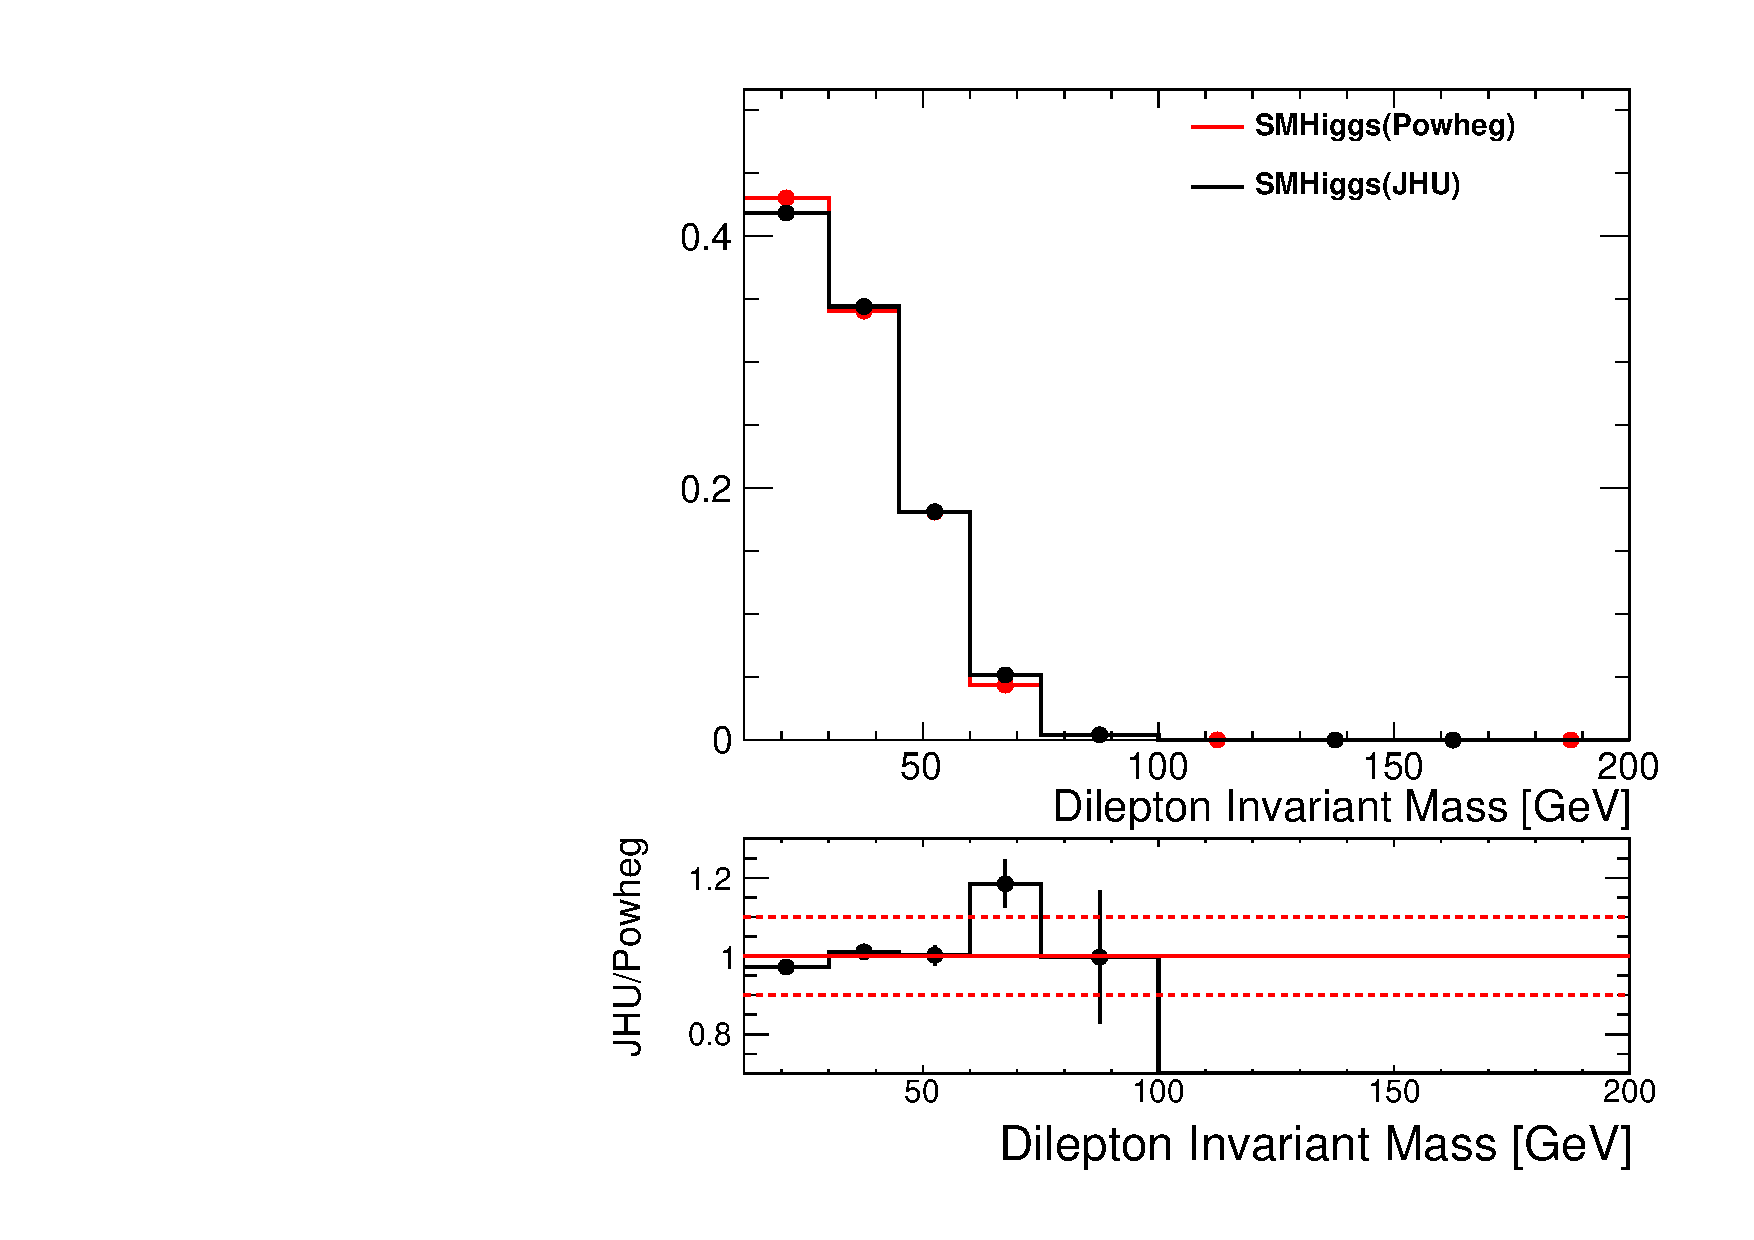
\includegraphics[width=.3\textwidth]{figures/mll.pdf}
} 
\subfigure[Transverse Higgs Mass]{
\centering
\label{subfig:mt}
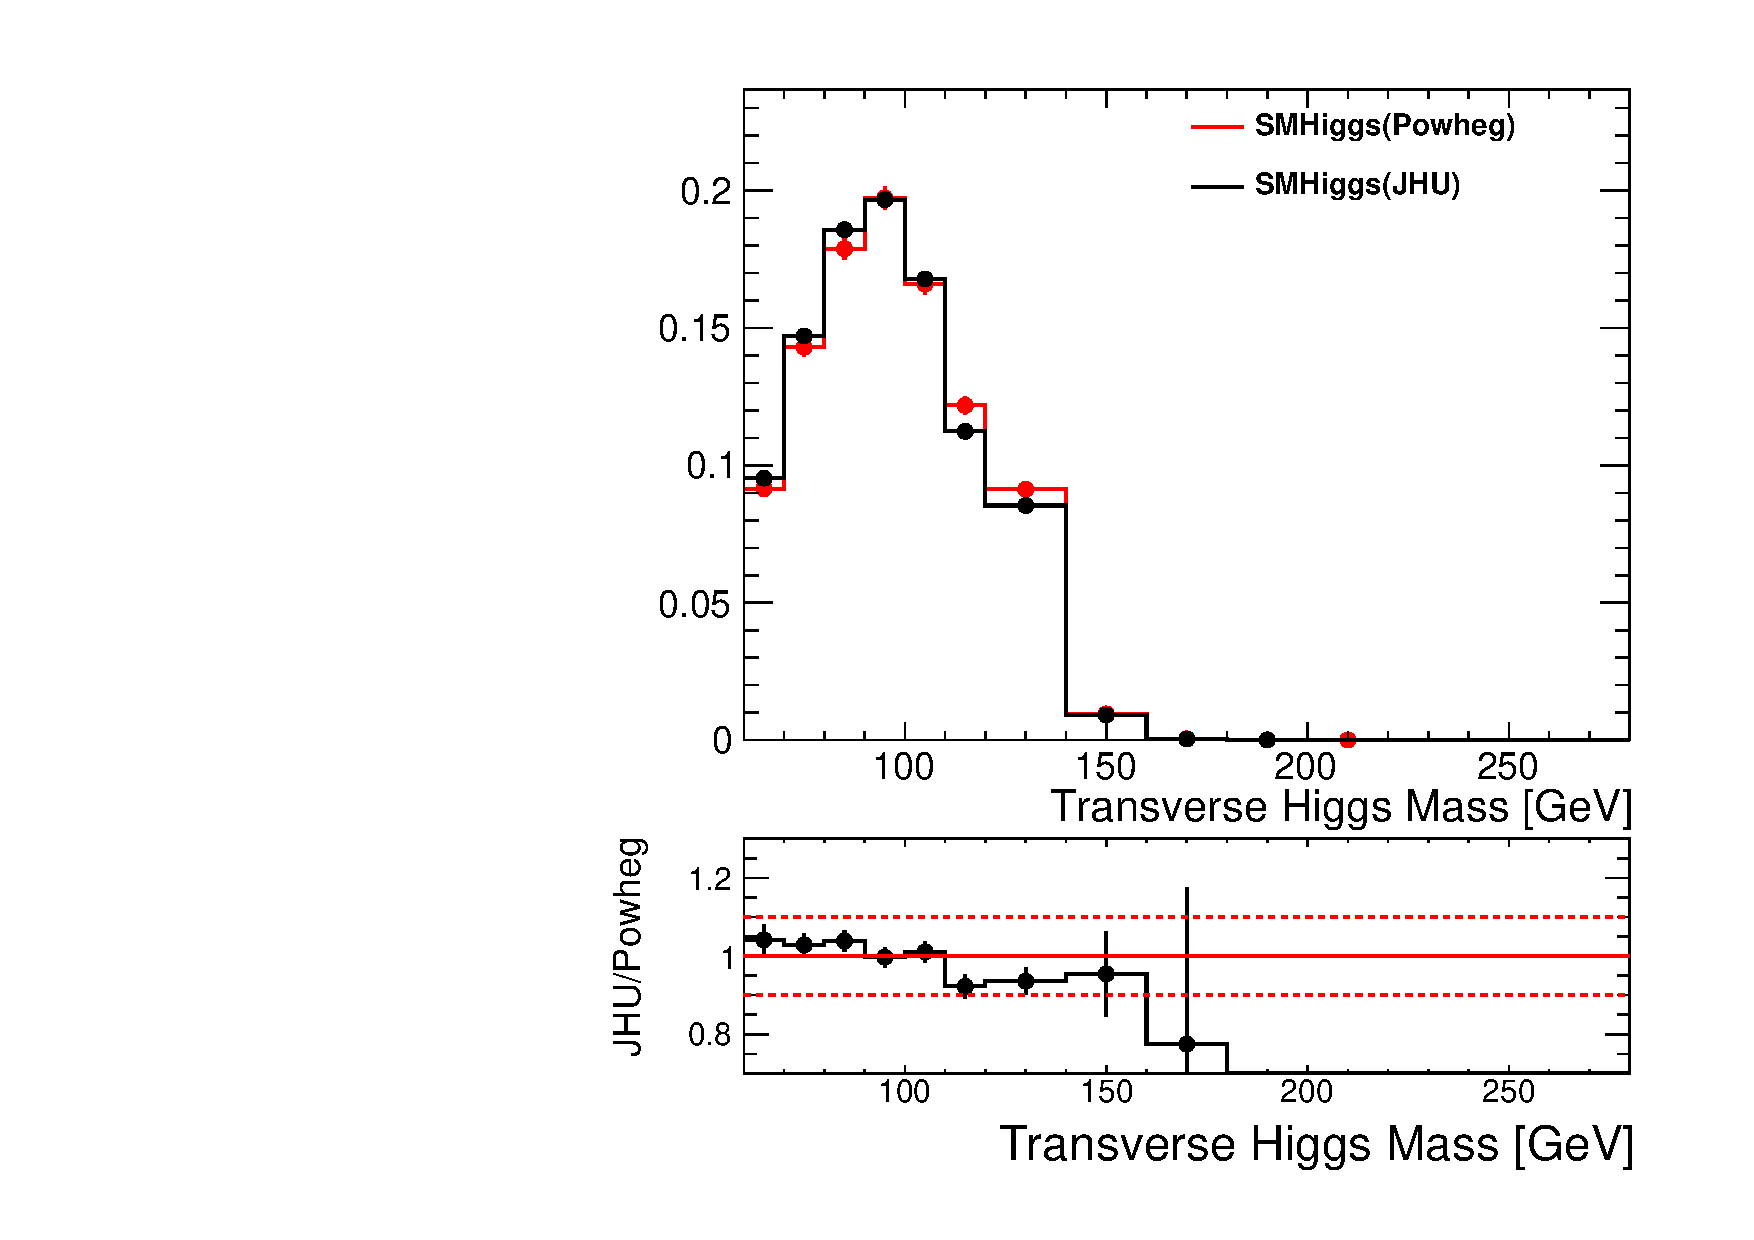
\includegraphics[width=.3\textwidth]{figures/mt.pdf}
}\\
\subfigure[Dilepton $p_T$]{
\centering
\label{subfig:dilpt}
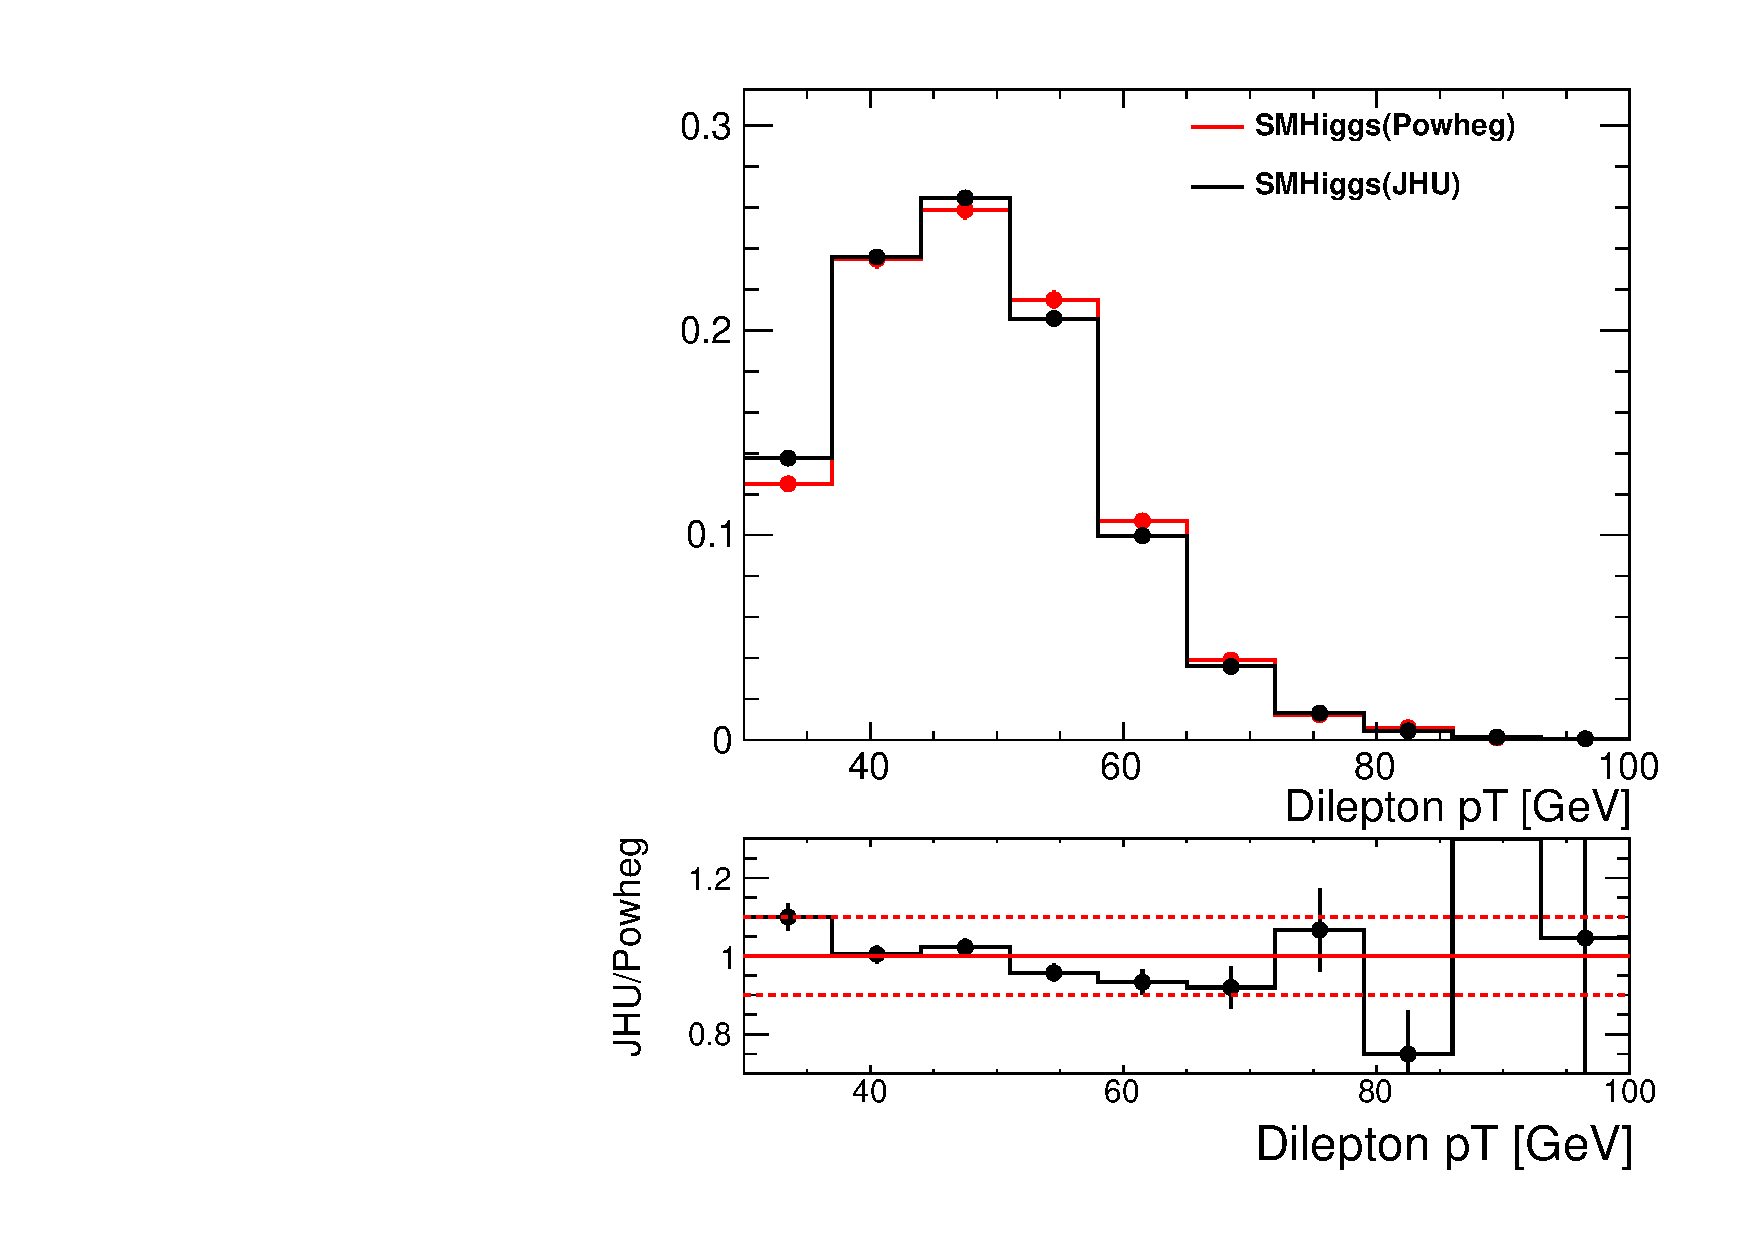
\includegraphics[width=.3\textwidth]{figures/dilpt.pdf}
}
\subfigure[Missing Energy]{
\centering
\label{subfig:met}
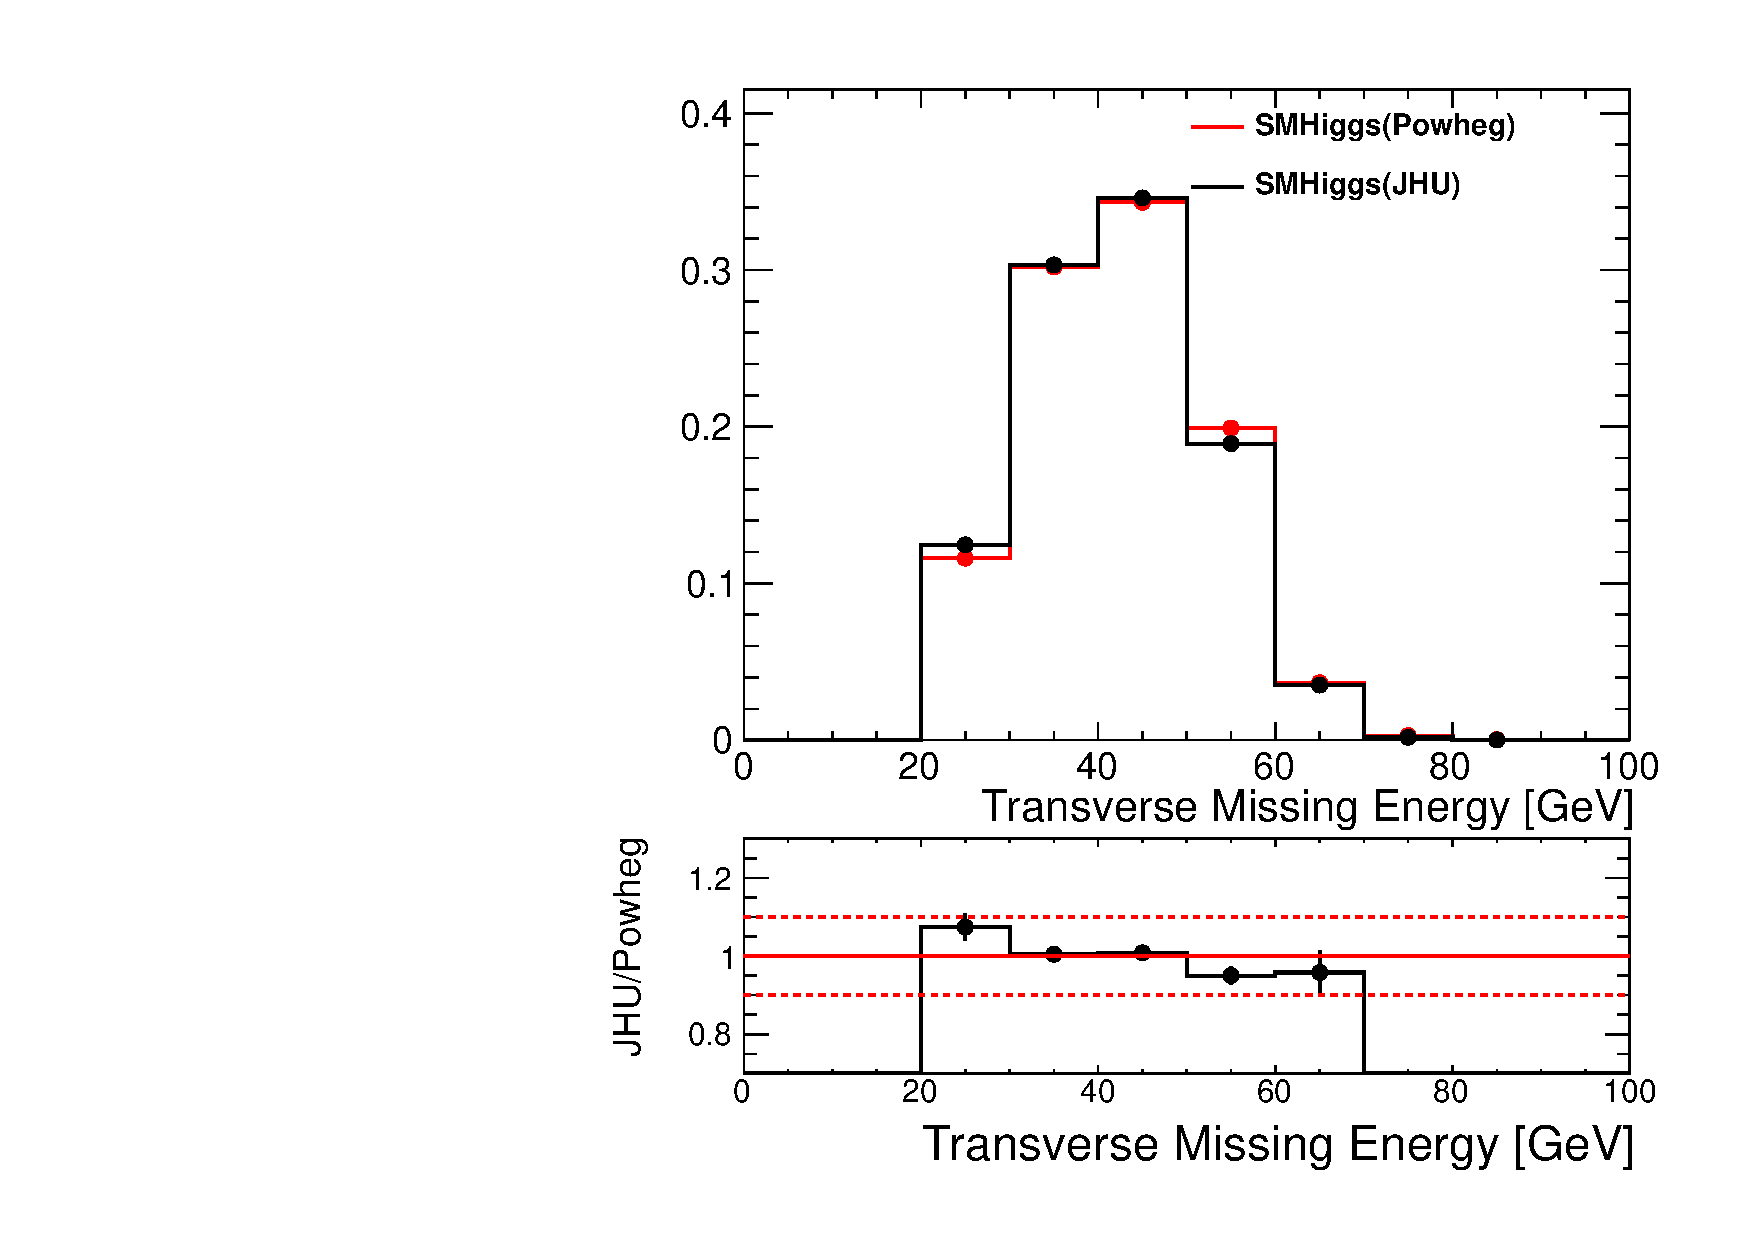
\includegraphics[width=.3\textwidth]{figures/met.pdf}
}
\subfigure[$\Delta\phi_{\ell\ell}$]{
\centering
\label{subfig:met}
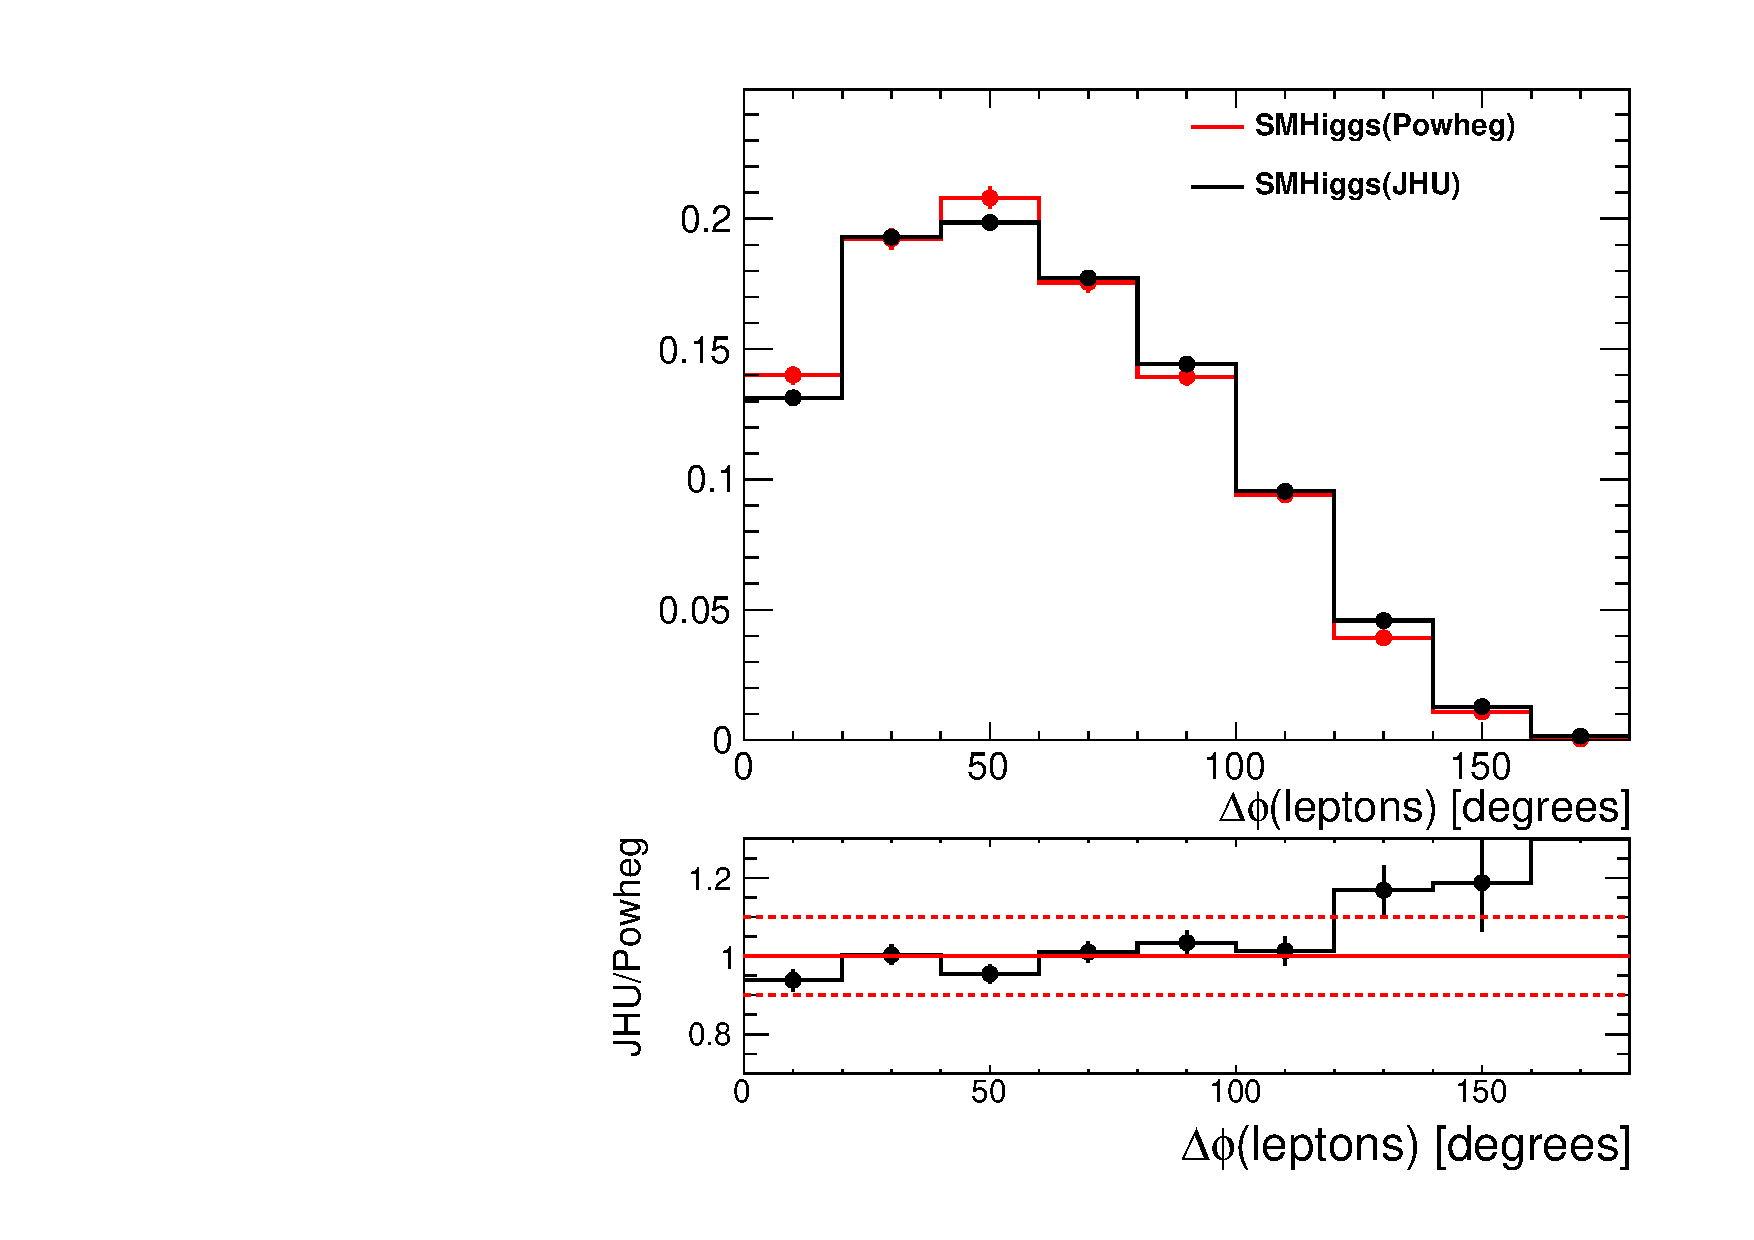
\includegraphics[width=.3\textwidth]{figures/dphill.pdf}
}\\
\caption{Kinematic distributions (normalized to 1) of the SM Higgs hypothesis 
comparing Powheg-Pythia and JHUGen-Pythia for reconstructed events 
after final event selections. }
\label{fig:higgskin_0j}
\end{figure}
%%%%%%%%%%%%%%%%%%%%%%%%%%%%%%%%%%%%%%%%%%%%%

%%%%%%%%%%%%%%%%%%%%%%%%%%%%%%%%%%%%%%%%%%%%%
\begin{figure}[!hbtp]
\centering
\subfigure[Higgs $p_T$]{
\centering
\label{subfig:higgspt_0j}
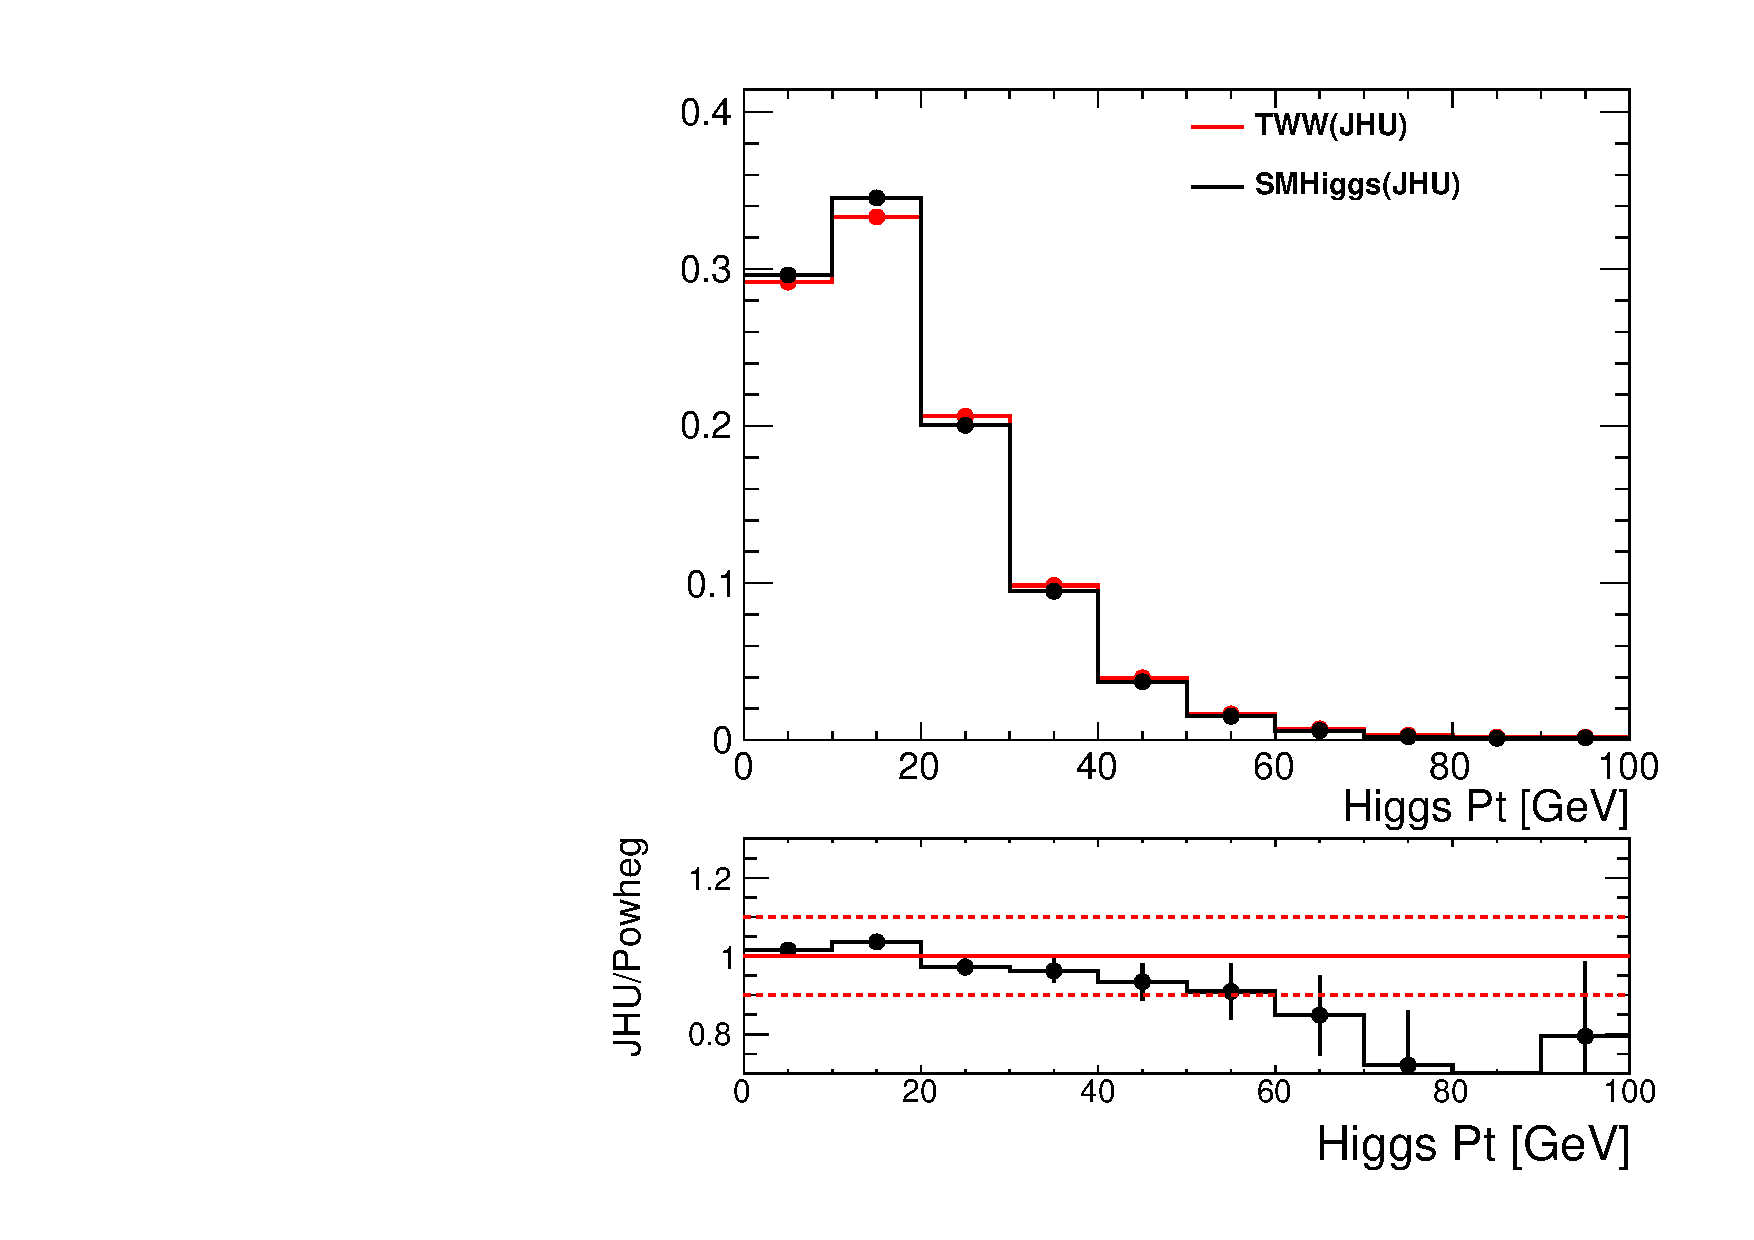
\includegraphics[width=.3\textwidth]{figures/higgsPt_gravitonvshiggs.pdf}
}
\subfigure[Leading Jet $p_T$]{
\centering
\label{subfig:jet1pt_0j}
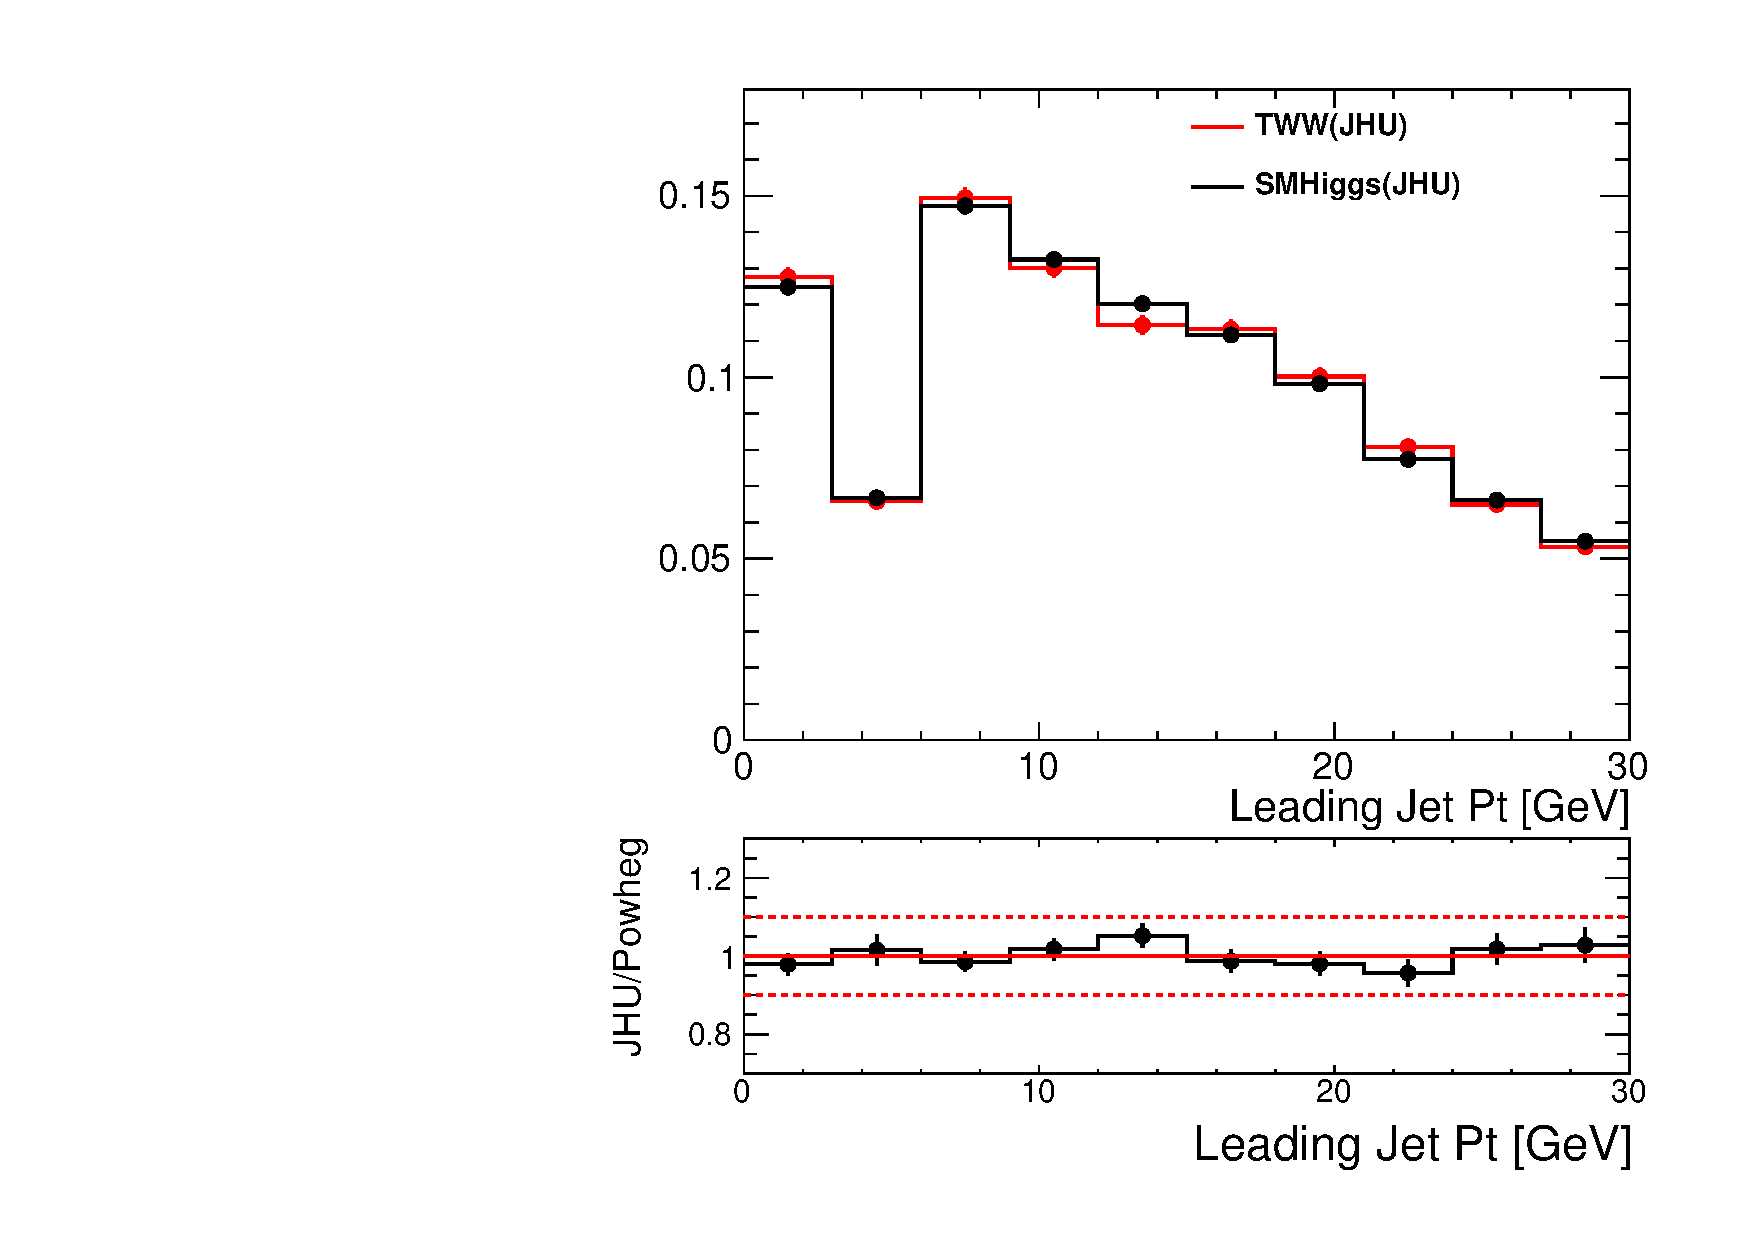
\includegraphics[width=.3\textwidth]{figures/jet1pt_gravitonvshiggs.pdf}
}\\
\caption{The Higgs $p_T$ and the leading jet $p_T$ distributions (normalized to 1) of the 
SM Higgs hypothesis compared to the Graviton ($2_m^+$) hypothesis, applying 
final event selections. }
\label{fig:gravvshiggspt_0j}
\end{figure}
%%%%%%%%%%%%%%%%%%%%%%%%%%%%%%%%%%%%%%%%%%%%%

